\documentclass[11pt,a4paper]{article}
\ifdefined\pdfminorversion\pdfminorversion=7\fi
\usepackage[T1]{fontenc}
\usepackage[utf8]{inputenc}
\usepackage{lmodern}
\usepackage[a4paper,left=2.35cm,right=2.35cm,top=2.25cm,bottom=2.15cm]{geometry}
\usepackage{amsmath}
\usepackage{graphicx}
\usepackage{array}
\usepackage{float}
\usepackage[section]{placeins}
\usepackage{needspace}
\usepackage{microtype}
\usepackage{cite}
\usepackage{xurl}
\usepackage[hidelinks]{hyperref}
\hypersetup{
  pdftitle={Soil Moisture Monitoring and Water Quantity Prediction},
  pdfauthor={Keolin Naicker, Lokadi Naicker, Arjun Ramphal, Darian Robert, Ntethelelo Shabalala}
}
\setlength{\emergencystretch}{1.5em}
\renewcommand{\arraystretch}{1.15}

\title{Soil Moisture Monitoring and Water Quantity Prediction}
\author{Keolin Naicker\\
Lokadi Naicker\\
Arjun Ramphal\\
Darian Robert\\
Ntethelelo Shabalala}
\date{COMP717A Contemporary Topics in Computer Science A\\
University of KwaZulu-Natal}

\begin{document}
\maketitle

\begin{abstract}
This project developed an IoT system that monitors soil moisture, predicts a water quantity for a selected target, and reports water use. A Grove Moisture Sensor v1.4 and Arduino Uno supplied readings to a Raspberry Pi 5, which ran a browser dashboard. Repeated tests with fresh soil samples established dry and wet references and measured the response to small water additions. Five retained training trials supplied the water-response curves. The dashboard estimated the water needed, suggested a measured portion, and used visual and optional audible dry warnings to attract the user's attention. Historical graphs linked recorded water additions to the soil response and compared predictions with measured totals. Daily and weekly summaries reported water use and the periods represented by saved readings. A displayed example estimated 5.9~mL and suggested a 2.0~mL portion. Applying the final method to the saved baseline of a separate check gave 6.1~mL, compared with 5.5~mL applied to reach the target. The system connected monitoring, measured watering, feedback and reporting to support careful water use and favourable growing conditions.
\end{abstract}

\noindent\textbf{Keywords:} soil moisture, water prediction, calibration, Arduino Uno, Raspberry Pi 5, IoT.

\section{Introduction}

Watering decisions affect both water use and the conditions around plant roots. Water spreads through soil pores, and its movement depends on the soil structure and moisture condition \cite{ref14}. A useful garden-monitoring system should therefore help the user recognise dry conditions, choose a measured amount of water and inspect the response after watering.

Soil-moisture sensors provide information that can support irrigation decisions and careful use of water \cite{ref4}. Combining these measurements with a dashboard makes the information easier to access. Adding a water-quantity estimate also helps the user move from recognising a dry condition to choosing a practical watering action.

This project brings these functions together. A moisture probe supplies measurements through an Arduino Uno to a Raspberry Pi 5. The dashboard shows the raw ADC reading, a calibrated relative moisture index and the watering status. Multiple soil trials supply the curves used to predict how much water is needed. The user adds water by hand, records the amount and checks the soil response. Visual and optional audible warnings draw attention to confirmed dry conditions. The history page connects recorded additions with the moisture trace, compares predicted and measured water quantities, and summarises daily and weekly water use.

\Needspace{8\baselineskip}
\subsection{Problem Definition and Objectives}

The practical problem was to guide watering using both the current soil condition and the measured response to earlier water additions. The work applies the wider garden-management objectives to water use. Its objectives were to:

\begin{enumerate}
\item Monitor soil conditions and indicate watering when needed, using visual and optional audible dry-soil warnings and a predicted quantity for a selected moisture target.
\item Support efficient water use through measured portions, feedback after watering and a clear stopping point, helping maintain conditions favourable to plant growth and prevent wastage.
\item Report soil condition, watering status, water-response and prediction results, daily and weekly water use, and user observations through a browser dashboard.
\end{enumerate}

Repeated testing with fresh soil was central to the project. It helped the team establish the moisture scale, examine the response to water and build the quantity-prediction feature. The complete process connects a soil measurement to a watering decision and a saved record of the action taken.

\section{Related Work}

\subsection{Moisture Sensors and Calibration}

The Grove v1.4 is a resistive moisture sensor. Its exposed probes respond to the electrical resistance of the surrounding soil \cite{ref6}. This provides a simple way to detect changes between dry and wet conditions. Reference readings from the sensor and soil give the output a useful scale for the application.

Chowdhury, Sen and Janardhanan compare low-cost resistive and capacitive sensors through calibration and water-response experiments \cite{ref2}. Their study separates two useful tasks: relating sensor readings to soil moisture, and observing the response when measured water is added. In their tests, the resistive sensor achieved a stronger calibration fit, while the capacitive sensor gave more consistent response measurements. Their findings support repeated trials when choosing and calibrating an inexpensive probe.

This distinction shaped the present work. The dry and wet references established the relative moisture index. Further trials recorded the index after measured water additions. Those water-response records then supplied the curves used by the prediction feature.

\subsection{Soil Conditions and Watering Decisions}

Zaman, Jain and F{\"o}rster investigate the use of low-cost sensors to estimate volumetric water content and field capacity \cite{ref3}. Volumetric water content describes the water volume within a soil volume. Field capacity describes the moisture remaining after excess water has drained away. The researchers used reference measurements and compared several trained models. Their results show how a measured sensor response can support useful estimates when an appropriate model and reference data are available.

The present system uses measured water additions and a relative moisture index to estimate the quantity needed to reach a selected target. It uses a straightforward calculation between recorded points, making the connection between the trial data and the displayed estimate easy to follow.

University of Minnesota Extension emphasises suitable placement, direct soil contact and calibration when using moisture sensors for irrigation scheduling \cite{ref4}. These factors also matter during repeated watering trials. Keeping the probe position and soil setup consistent helps the recorded response remain useful for later decisions. The guidance also connects moisture monitoring with irrigation management, which supports the project's focus on measured watering and recorded input use.

\subsection{A Related IoT Prototype}

Akb{\i}y{\i}k, Mammadova and Mamishova describe a moisture-monitoring prototype using an HW-103 probe, an Arduino Nano and a Raspberry Pi 5 \cite{ref5}. Their Arduino sends readings through a serial connection, and a Streamlit interface displays the moisture information. Dry and wet references provide a relative scale, while a threshold indicates when watering is required. Their results demonstrate the practical link between sensing, communication and visible watering guidance.

The present project follows that sensing-to-dashboard approach with a Grove v1.4, an Arduino Uno and Flask. It extends the watering guidance by learning from repeated water-addition trials, displaying an estimated quantity and recording the water applied. The reviewed work therefore supports the main design: calibrated sensing, clear warnings, repeated physical tests and a readable interface for the user.

\section{System Design and Technology Choices}

\subsection{Three-Layer IoT Architecture}

The prototype follows the three-layer Core IoT Functional Stack. Figure~\ref{fig:architecture} maps the equipment and software to the things, communications network and applications layers.

\begin{figure}[htbp]
\centering
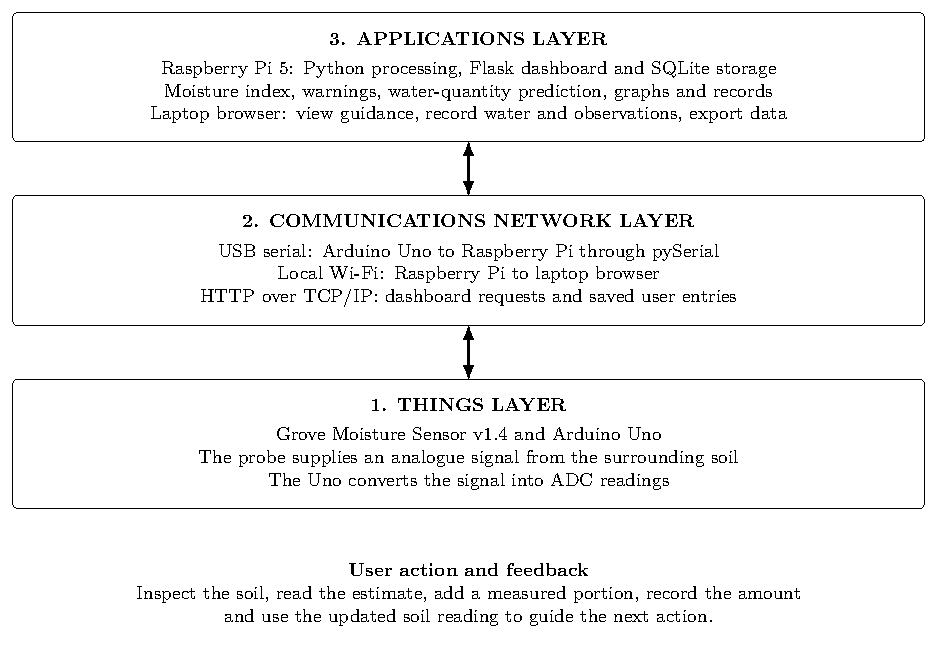
\includegraphics[width=.98\linewidth]{figures/module_architecture.pdf}
\caption{The prototype mapped to the three-layer Core IoT Functional Stack.}
\label{fig:architecture}
\end{figure}

The \textbf{things layer} contains the Grove moisture probe and Arduino Uno. The probe produces an analogue signal, and the Uno converts it into a digital ADC reading. The \textbf{communications network layer} carries readings over USB serial from the Uno to the Pi. Wi-Fi connects the Pi to the laptop browser, which accesses the dashboard through HTTP over TCP/IP.

The \textbf{applications layer} processes and stores the readings on the Pi. It calculates the moisture index, applies the warning rules and predicts a water quantity from the trial curves. The dashboard presents live information, accepts water entries and observations, and provides exports. Its history views display the response to recorded additions, compare predictions with measured totals, and calculate daily and weekly summaries. The browser produces the optional warning sound through the viewing device's speakers. The user completes the physical watering action and checks the resulting measurements.

\subsection{Components and Reasons for Their Selection}

The Uno provides analogue inputs and a 10-bit ADC, giving readings from 0 to 1023 \cite{ref9}. This makes it suitable for the probe's analogue output. The Raspberry Pi provides a Linux computer with USB and networking for data collection and the web application \cite{ref17}.

\begin{table}[htbp]
\centering
\caption{Main components and their roles}
\label{tab:components}
\begin{tabular}{|>{\raggedright\arraybackslash}p{4.0cm}|>{\raggedright\arraybackslash}p{10.7cm}|}
\hline
\textbf{Component} & \textbf{Role and reason for use} \\ \hline
Grove Moisture Sensor v1.4 & Supplies a changing analogue signal for soil-moisture monitoring. \\ \hline
Arduino Uno & Reads the sensor through A0, selects a median measurement and sends it over USB. \\ \hline
Raspberry Pi 5 and microSD & Run the application and keep the database locally. \\ \hline
Grove cable and jumpers & Connect the probe's power, ground and signal to the Uno. \\ \hline
USB-A to USB-B cable & Carries measurements to the Pi and supplies power to the Uno. \\ \hline
Flask and Waitress & Provide the browser application and its web server. \\ \hline
pySerial and SQLite & Receive serial measurements and store readings, trial points and water entries. \\ \hline
5~mL syringe & Measures water additions using its 0.5~mL graduations. \\ \hline
\end{tabular}
\end{table}

Python suited the processing and prediction calculations. Flask provided the dashboard, and Waitress served the application \cite{ref10}. pySerial supported communication with the Uno \cite{ref11}. SQLite, accessed through Python, kept measurements and water records in a local database \cite{ref12}. This combination supported one continuous collector and a dashboard that could be viewed from the laptop.

\subsection{Wiring and Physical Setup}

The sensor's red wire connected to Uno 5V, black to GND and yellow to A0. The white wire remained disconnected. The USB cable connected the Uno to the Pi. A separate USB-C power source supplied the Pi. Figure~\ref{fig:wiring} shows the connections, and Figure~\ref{fig:hardware} shows the assembled prototype.

\begin{figure}[htbp]
    \centering
    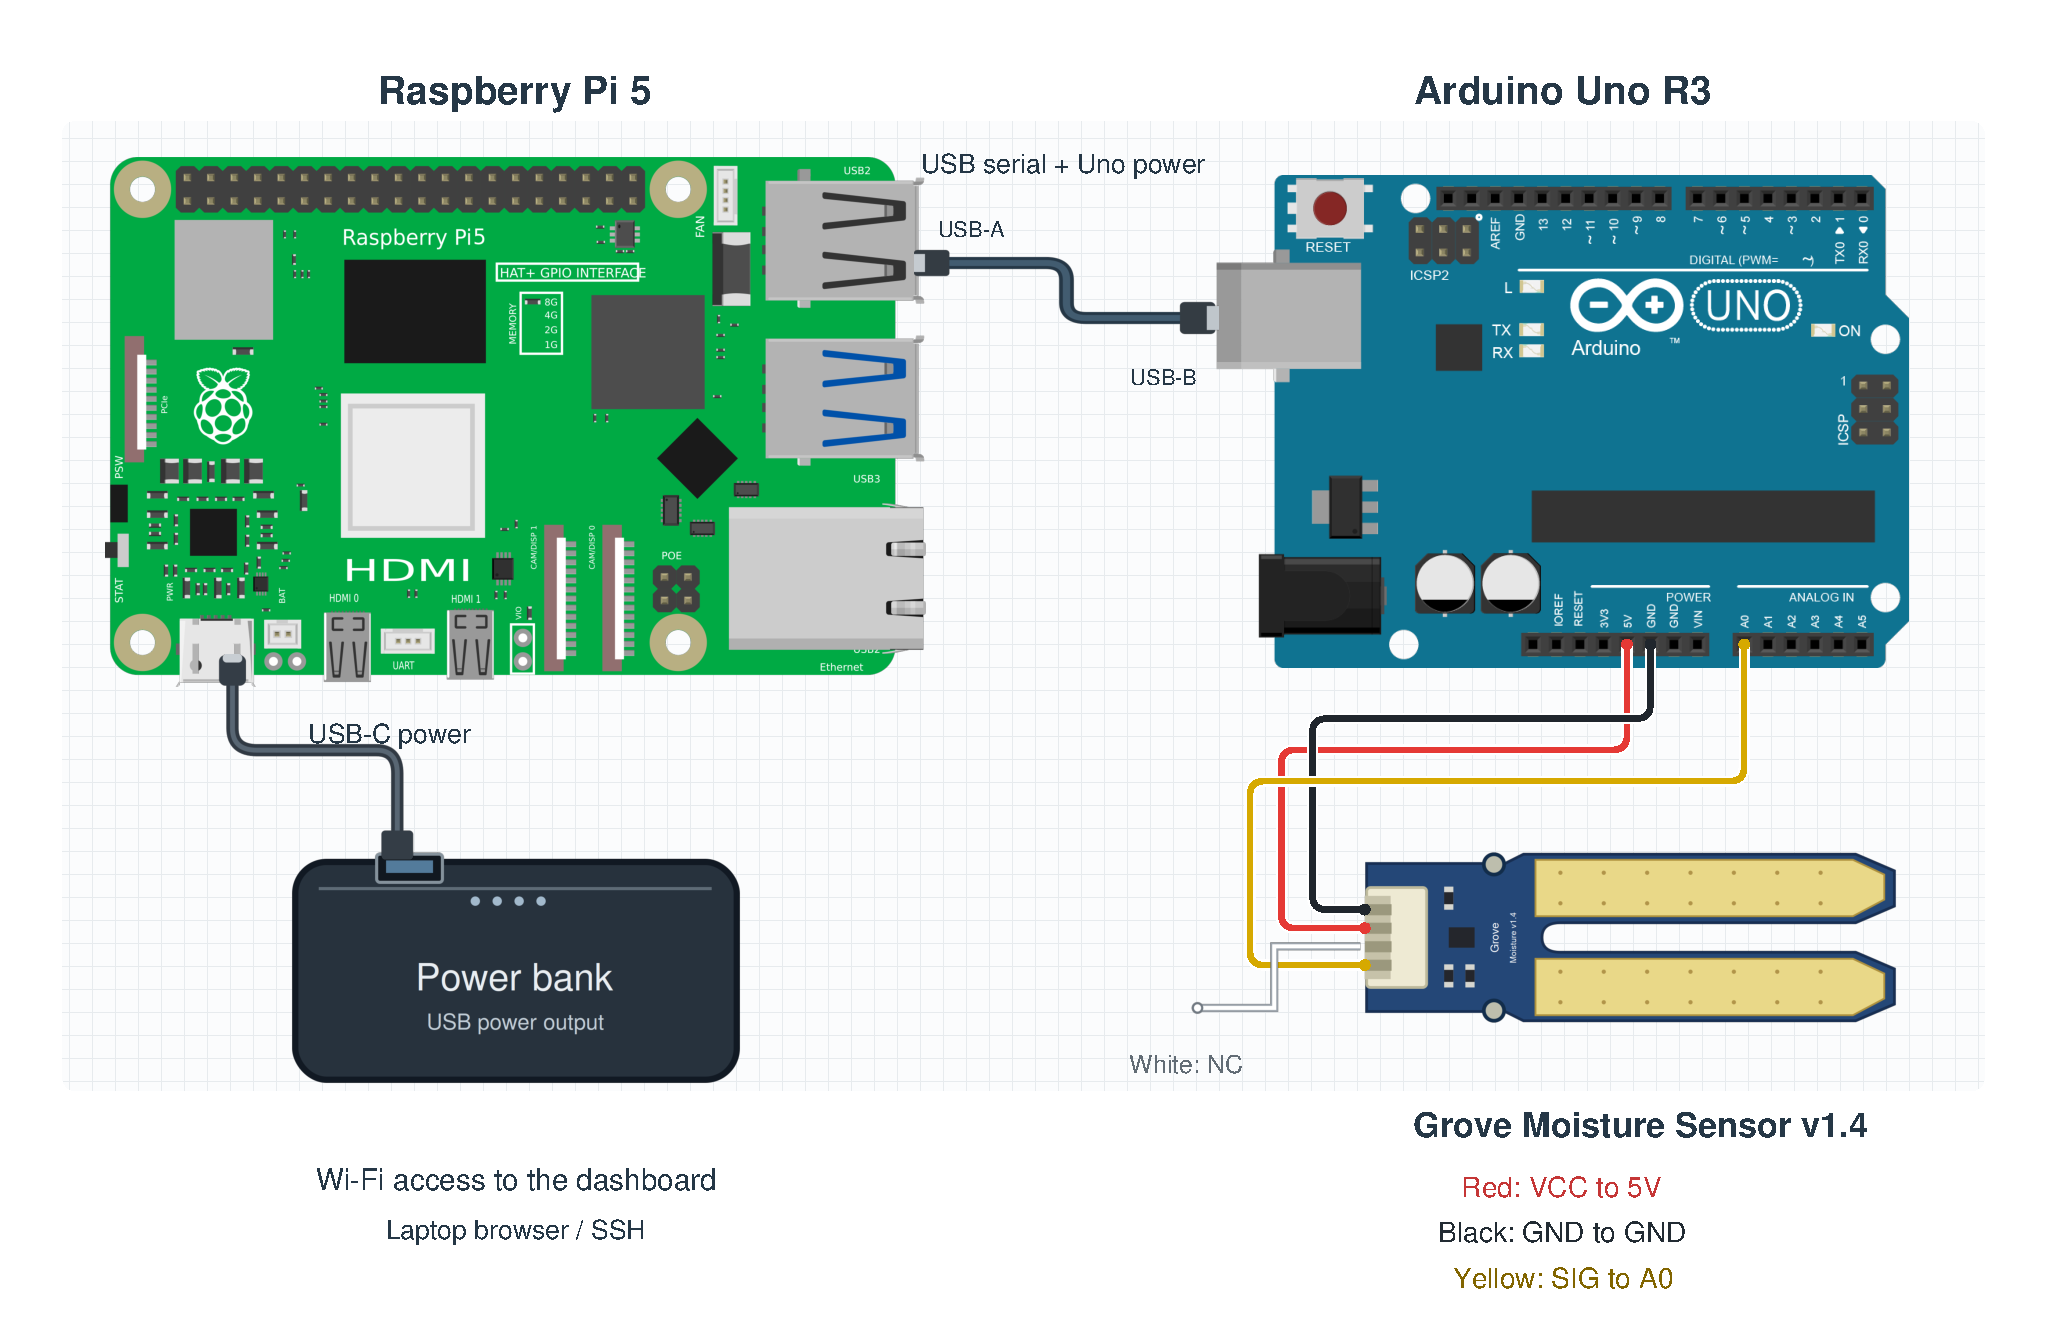
\includegraphics[width=\linewidth]{figures/prototype_wiring.pdf}
    \caption{Hardware connections of the prototype, showing the Grove
    v1.4 moisture sensor, Arduino Uno, Raspberry Pi 5 and USB power source.}
    \label{fig:wiring}
\end{figure}

\begin{figure}[htbp]
\centering
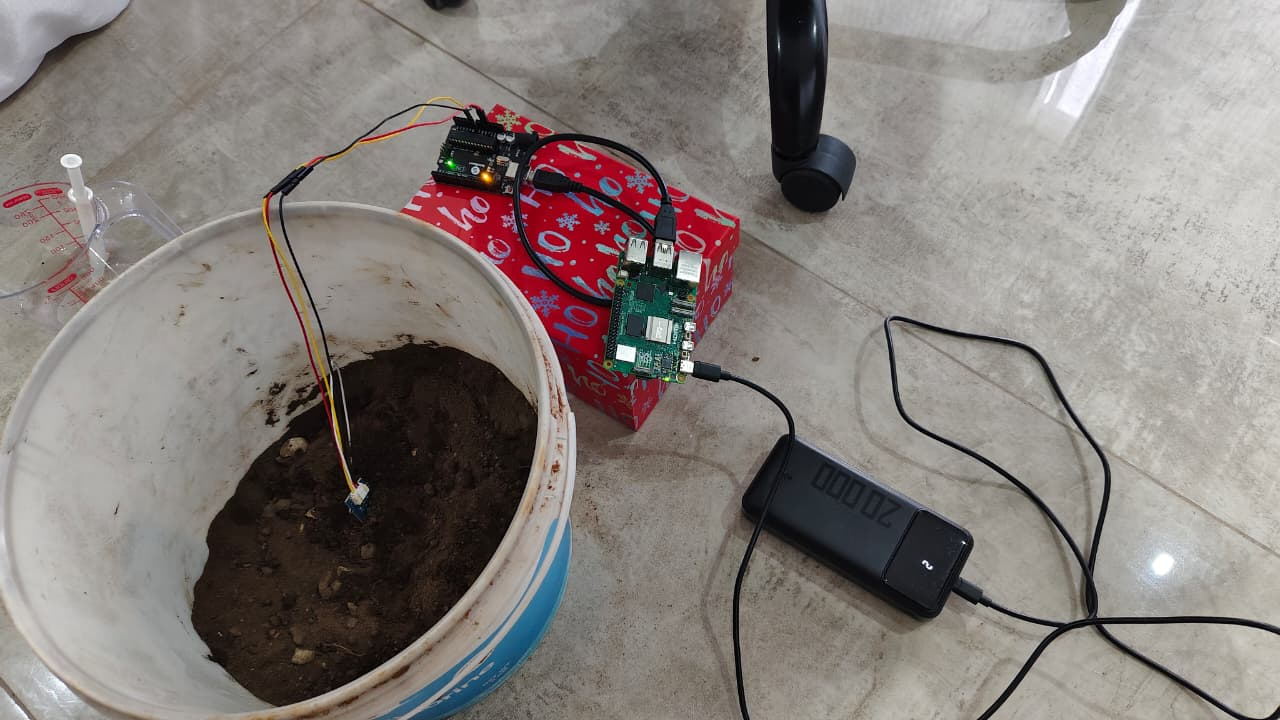
\includegraphics[width=\linewidth]{figures/wiring_real.jpeg}
\caption{The physical prototype with the soil container, Uno, Pi and power source.}
\label{fig:hardware}
\end{figure}

The Pi was operated headlessly, with the laptop providing remote access over the local network. The probe was placed in the soil at a recorded depth of 3.75~cm. Water was measured with the syringe and applied around the probe during the trials.

\section{Implementation and Experimental Procedure}

\subsection{Acquiring and Displaying Readings}

The Uno read the sensor through A0. Each reported value was the median of nine ADC measurements. Selecting the middle reading reduced the effect of a brief spike within the measurement group. The Uno sent the readings to the Pi over serial communication at 115200 baud.

The system collected approximately one reading per second. A background collector handled the serial connection, while the browser requested updated information. The Live dashboard page displayed raw ADC, relative moisture index, warning status, connection information and the total water recorded. The History \& results page read the saved measurements and water ledger to show response graphs, prediction comparisons and summaries. Both pages provided controls for the optional audible dry warning.

\subsection{Moisture Calibration with Fresh Soil}

The team repeated dry and wet tests using fresh soil samples. The probe depth and position were kept consistent within each trial. This required practical adjustment of the soil contact and patience while readings settled. Figure~\ref{fig:soil} shows the probe placement.

\begin{figure}[htbp]
\centering
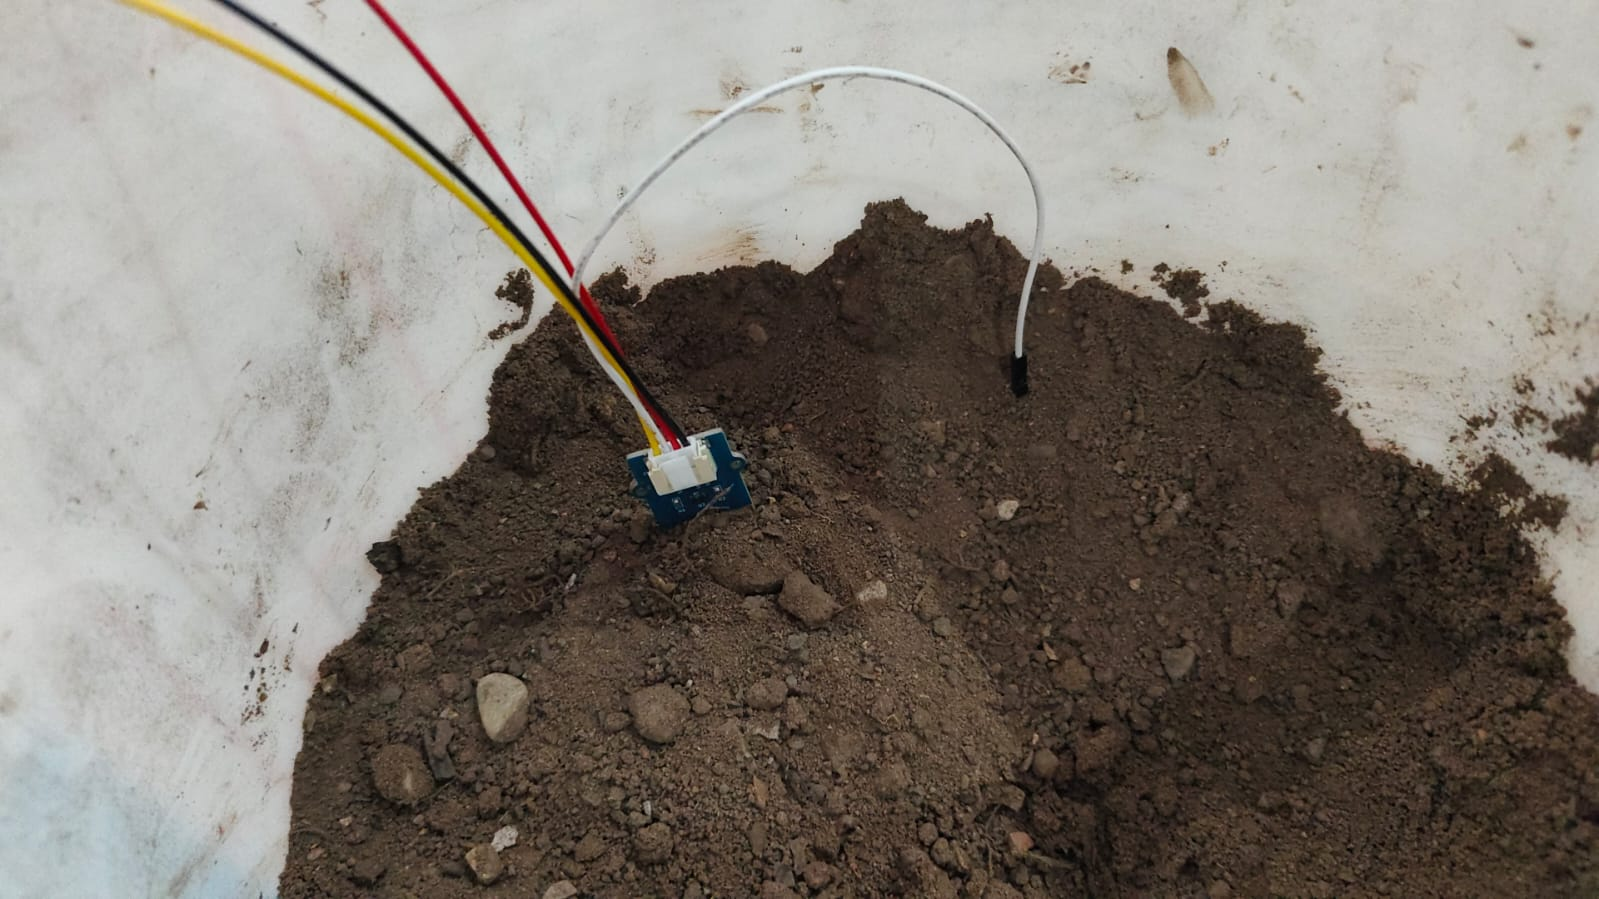
\includegraphics[width=.72\linewidth]{figures/soil_sample.jpeg}
\caption{The moisture probe placed in a soil sample for calibration and watering tests.}
\label{fig:soil}
\end{figure}

For each reference capture, the application took the median of 12 recent readings. The selected dry and wet values defined the working scale. Let $A$ be the current ADC value, $D$ the dry reference and $W$ the wet reference. The relative moisture index was:

\begin{equation}
I=\min\left(100,\max\left(0,\frac{100(A-D)}{W-D}\right)\right).
\label{eq:index}
\end{equation}

The index runs from 0 to 100 and shows the reading's position between the two references. The team used this scale to set the dry warning and the watering target.

\subsection{Warnings and Watering Rules}

Selecting the warning limits required several rounds of testing and adjustment. We tested fresh soil samples and compared the ADC readings, relative moisture index and dashboard messages with the observed soil
condition. Measured water additions helped us examine how the readings
changed as the soil became wetter. Different warning and clearing settings
were tried before the final values were selected.

The dry-warning limit was set to index 30 to prompt the user to inspect
the soil when the reading entered the lower part of the calibrated scale.
The clearing limit was set to index 60 so that the warning would remain
active until a clear increase in the reading had occurred. Index 60 also
became the target used by the water-quantity prediction. These settings
were chosen for the soil and sensor setup used in the project.

Three successive readings at or below index 30 raised a dry-soil warning.
Once active, the warning cleared after three successive readings at or
above index 60. Between these limits, the current warning state was
retained. Using separate warning and clearing limits is called hysteresis.
Together with the three-reading confirmation rule, this reduced repeated
switching caused by small changes in the sensor reading.

Saving a water addition started a three-minute soak pause. During this pause, the user allowed the water to spread. The application then required a settled reading before offering the next portion. These steps helped connect the advice to the soil response.

The browser provided an optional audible warning alongside the visual message. Selecting \emph{Enable sound} allowed a three-note chime when a fresh sensor reading produced a confirmed dry-warning state. The chime repeated every 30 seconds while that state remained active. \emph{Silence this warning} acknowledged the current warning, while a later warning could sound again. The chime stopped during the soak pause or when the system reported a sensor or connection problem.

Figure~\ref{fig:audible-warning} shows the sound controls. \emph{Test sound} played the chime on request, and \emph{Disable sound} turned the audible warning off. Sound came from the laptop or phone displaying the dashboard. The user enabled it in the browser tab kept open for monitoring.

\begin{figure}[htbp]
\centering
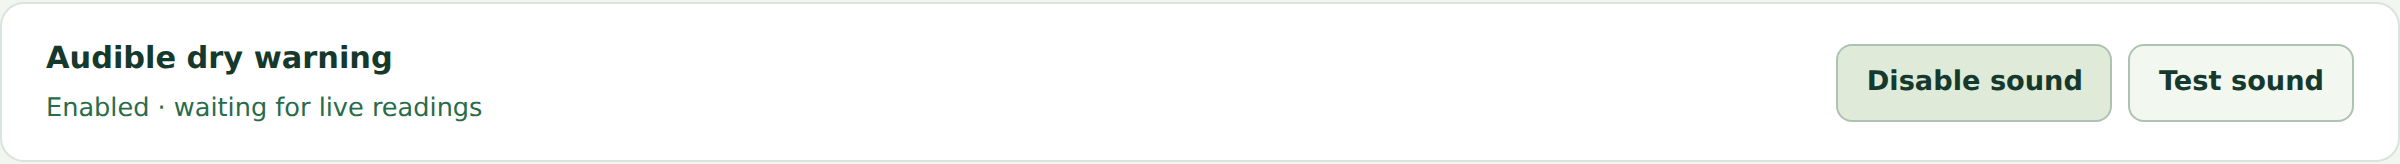
\includegraphics[width=\linewidth]{figures/audible_dry_warning.png}
\caption{Browser controls for the audible dry warning. Sound is enabled in this capture, with the displayed state waiting for live readings.}
\label{fig:audible-warning}
\end{figure}

\begin{table}[htbp]
\centering
\caption{Settings used for monitoring and water-quantity guidance}
\label{tab:settings}
\begin{tabular}{|>{\raggedright\arraybackslash}p{8.6cm}|>{\raggedright\arraybackslash}p{6.1cm}|}
\hline
\textbf{Setting} & \textbf{Value} \\ \hline
Dry and wet ADC references & 0 and 636 \\ \hline
Dry-soil warning threshold & Index 30 \\ \hline
Warning clearing and watering target & Index 60 \\ \hline
Confirmation for warning changes & 3 successive readings \\ \hline
Maximum suggested water portion & 2.0~mL \\ \hline
Measurable portion increment & 0.5~mL \\ \hline
Selected check-error allowance & 2.0~mL \\ \hline
\end{tabular}
\end{table}

\subsection{Learning the Response to Measured Water}

Water calibration used repeated wetting trials with fresh soil. Each trial began with a settled starting index and a cumulative water amount of zero. The user then added a measured portion, recorded it, allowed the soak pause to finish and captured the settled reading. This sequence continued until the target index was reached.

Each captured point paired the total water added with the settled moisture index. The full water total was kept even when an early portion produced little change in the sensor reading. This was important because later changes could depend on water already spreading through the soil.

Five retained training trials supplied the response curves. For calculation, small falls in a trial's index were handled by keeping the highest settled value reached so far. All measured points remained available in the records. The resulting curves linked increasing water totals to the observed moisture response.

\subsection{Predicting a Water Quantity}

The final method compared the increase in index needed by a new sample with the increases recorded in the training trials. If the sample started at index $S$ and the target was $T$, the required increase was $T-S$. For each training trial, this increase was added to that trial's own starting index. The application then read the cumulative water amount at the resulting position on its curve.

When the required position fell between two measured points, the application used a straight-line estimate between them. Only trials covering the required increase contributed. At least three suitable trial estimates were required, and their spread was checked against the selected agreement limit. Their median gave the starting water estimate, $V_0$.

For example, a starting index near 6.4 and a target of 60 required an increase of about 53.6 points. Four training curves covered that increase. Their estimates gave a median of about 5.9~mL.

The application kept this starting estimate for the current soil sample and subtracted the water actually recorded:

\begin{equation}
V_{\mathrm{remaining}}=\max\left(0,V_0-V_{\mathrm{recorded}}\right).
\label{eq:remaining}
\end{equation}

The next suggested portion was approximately half the remaining estimate, rounded down to a measurable 0.5~mL increment and capped at 2.0~mL. A 5.9~mL estimate therefore began with a 2.0~mL portion. In a worked calculation, recording that portion left about 3.9~mL, with a next portion of 1.5~mL. Reaching the moisture target ended the watering guidance. \emph{New soil sample} was selected when replacing the soil, so each sample began with its own starting estimate and water record.

\subsection{Using the Dashboard}

The dashboard provided a Live dashboard page for current decisions and a History \& results page for reviewing saved records. The watering process followed these steps:

\begin{enumerate}
\item Check the ADC, relative index and watering status. Enable sound if an audible dry warning is wanted.
\item Inspect the soil when the dry warning appears.
\item Read the estimated remaining water and the suggested next portion.
\item Measure and add that portion, then record the actual amount applied.
\item Allow the soak pause to finish and wait for a settled reading.
\item Continue with the updated guidance, stopping when the target is reached.
\item Review the recorded water response, prediction results and water-use summaries on the history page.
\end{enumerate}

Figure~\ref{fig:workflow} summarises this measurement-and-feedback process. When readings were old, missing or unstable, the interface asked the user to check the connection or wait for a reliable reading. The recent-events feed also made changes in the system state visible.

\begin{figure}[H]
\centering
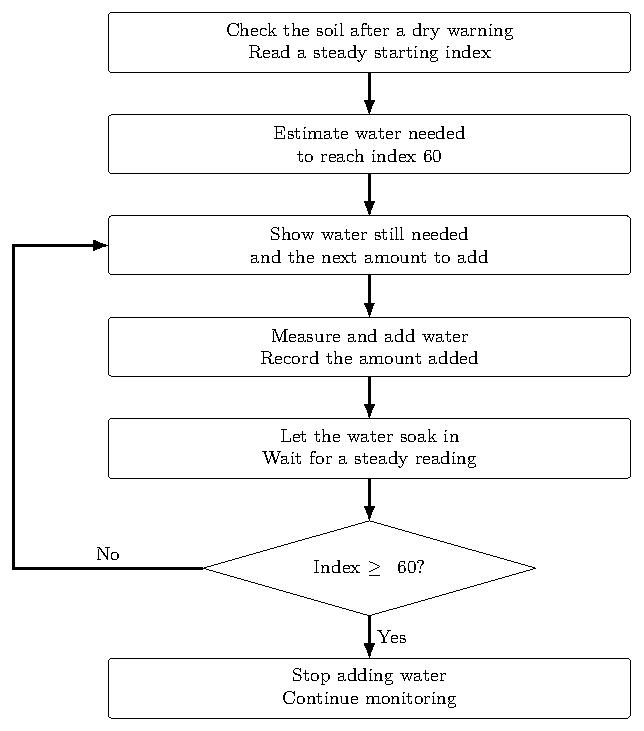
\includegraphics[width=.85\linewidth]{figures/watering_workflow.pdf}
\caption{Watering guided by moisture measurements, a trained quantity estimate and feedback after each portion.}
\label{fig:workflow}
\end{figure}

\subsection{History Graphs and Water-Use Summaries}

The watering-response view combined the saved moisture trace with markers for each recorded water addition and the settled captures from a selected trial. Each marker showed the entered volume at its logging time. The user could select an individual run or all watering records for a chosen day. Lines stopped at missing intervals and changes of stream or calibration, keeping separate measurement sequences visible.

The prediction-results view compared an estimated volume with the total water physically recorded in a completed check. It showed the starting index, final index, target and absolute difference between the estimate and that total. \emph{Recorded checks} displayed the prediction saved when each check began. \emph{Saved recalculations} displayed stored calculations using the existing check measurements. Keeping these views separate preserved the meaning of each result.

Daily and weekly summaries grouped water entries using the South African calendar day and a Monday-to-Sunday week. They showed recorded water, entry count, recorded coverage and dry-warning time. Coverage counted intervals between consecutive readings in the same stream and calibration, within the allowed gap. Dry-warning time counted valid recorded intervals in the confirmed warning state. Missing intervals were excluded from both durations.

The weekly bar chart grouped water by its saved labels: training, checks, reference calibration and other records. The summaries therefore provided a period-based view of the water ledger alongside the detailed trial records.

\subsection{Records Used for Evaluation}

The evaluation used five retained training trials and two completed separate check runs. Trials that continued the same physical soil test were combined into one water-response sequence, keeping every addition in the cumulative total. This preserved the relationship between the original dry sample and all the water applied to it.

The final prediction method was also recalculated from the saved starting point of a separate check run and compared with that run's measured water response. The check measurements remained separate from the training curves. Results were examined through the captured trial points, warning states, water ledger and dashboard displays. The history graphs and summaries were checked against those saved records, linking each plotted water amount and reported total to its underlying entries.

\section{Results and Discussion}

\subsection{Dry and Wet References}

Repeated calibration produced working references of 0 and 636 ADC. Table~\ref{tab:calibration} summarises the captures used to establish the index.

\begin{table}[htbp]
\centering
\caption{Selected moisture-reference captures}
\label{tab:calibration}
\begin{tabular}{|l|c|c|}
\hline
\textbf{Reference} & \textbf{Median ADC} & \textbf{Captured ADC range} \\ \hline
Dry soil & 0 & 0--2 \\ \hline
Wet soil & 636 & 636--654 \\ \hline
\end{tabular}
\end{table}

With these references, 49 ADC corresponded to about 7.7 index points,
while 382 ADC corresponded to about 60.1 points. These readings illustrated
the dry-warning region and the selected clearing level.
Figure~\ref{fig:dry-warning-state} shows an active dry-soil warning,
while Figure~\ref{fig:monitoring-state} shows the monitoring state.
These screenshots document the reference-calibration stage. The water-quantity panel and history views are presented in the following results sections.
The stored calibrated readings agreed with Equation~\eqref{eq:index}.

\begin{figure}[H]
    \centering
    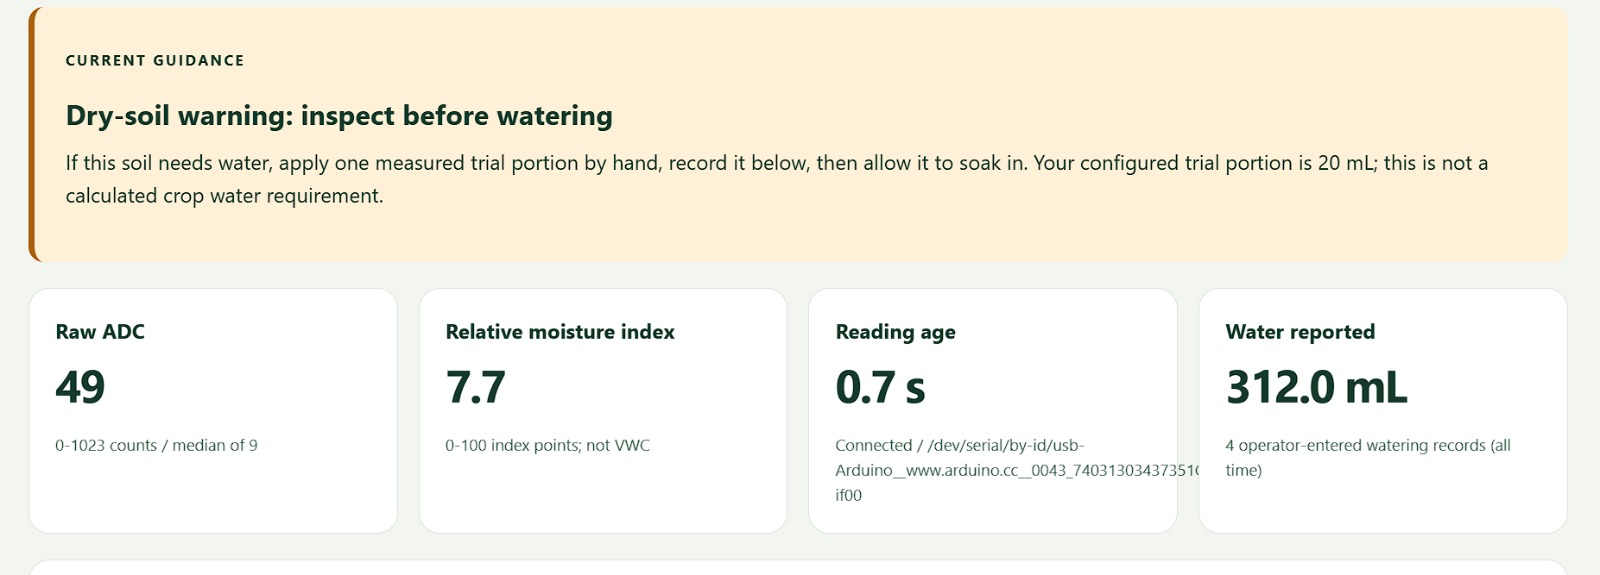
\includegraphics[width=\linewidth]{figures/dry_warning.jpeg}
    \caption{Calibration-stage capture of an active dry-soil warning at 49 ADC and an index of 7.7. The visible 20~mL trial instruction belongs to that calibration stage.}
    \label{fig:dry-warning-state}
\end{figure}

\begin{figure}[H]
    \centering
    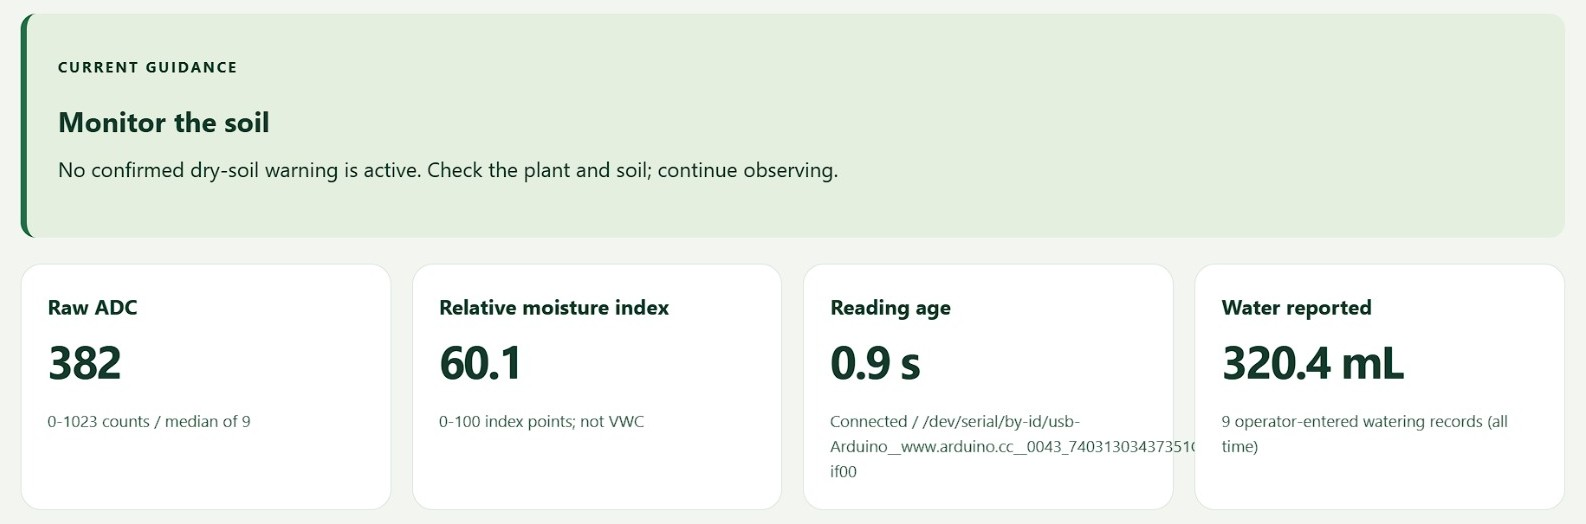
\includegraphics[width=\linewidth]{figures/monitoring.jpeg}
    \caption{Calibration-stage capture of the monitoring state at 382 ADC and an index of 60.1. The capture retains the labels shown during that test.}
    \label{fig:monitoring-state}
\end{figure}

\subsection{Response Across the Training Trials}

Table~\ref{tab:training} shows the five training trials used by the final water-prediction feature. Each reached the selected target after a sequence of measured additions. The cumulative totals ranged from 6.0 to 8.0~mL.

\begin{table}[H]
\centering
\caption{Retained training trials and their measured endpoints}
\label{tab:training}
\begin{tabular}{|c|r|r|r|}
\hline
\textbf{Trial} & \textbf{Starting index} & \textbf{Final index} & \textbf{Total water (mL)} \\ \hline
9 & 15.4 & 65.0 & 7.0 \\ \hline
10 & 6.9 & 65.7 & 8.0 \\ \hline
12 & 2.8 & 64.2 & 7.0 \\ \hline
13 & 0.5 & 62.4 & 6.0 \\ \hline
15 & 1.4 & 61.6 & 6.0 \\ \hline
\end{tabular}
\end{table}

Figure~\ref{fig:training} plots the captured moisture index against the total water added. The curves show why repeated fresh-soil trials were useful. Early portions sometimes produced only a small change, followed by a clearer rise as further water spread through the sample.

\begin{figure}[H]
\centering
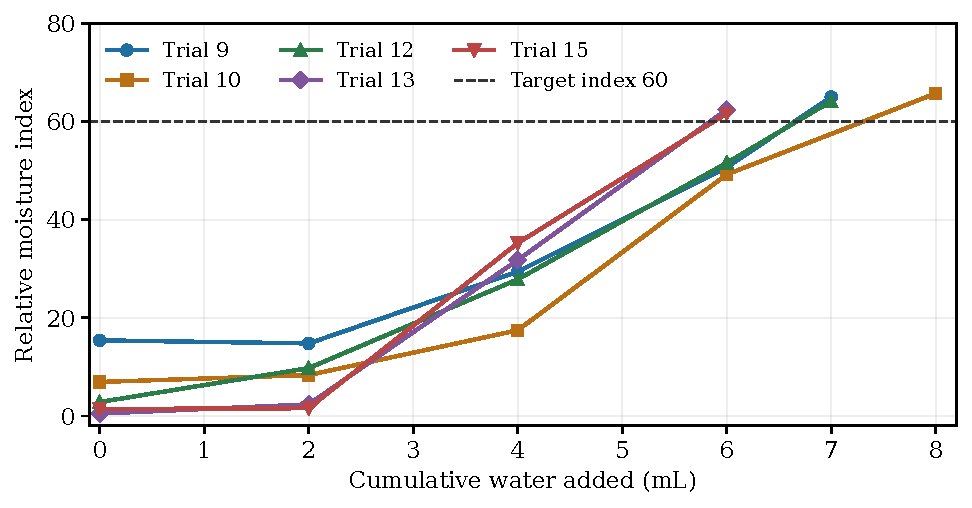
\includegraphics[width=\linewidth]{figures/training_response.pdf}
\caption{Measured water-response points from the five retained training trials. The dashed line marks the target index of 60.}
\label{fig:training}
\end{figure}

Trial 15 illustrates the importance of counting the full water history. Its index changed from about 1.4 to 1.6 after the first 2.0~mL. At a total of 4.0~mL, the index reached 35.2, and at 6.0~mL it reached 61.6. The complete sequence allowed the prediction curve to account for the early water as well as the later rise. The repeated trials therefore supplied a practical basis for estimating a quantity and choosing smaller portions as the target approached.

\subsection{Displayed Water Prediction}

The dashboard example in Figure~\ref{fig:prediction} shows a 5.9~mL remaining estimate, a 2.0~mL next portion and a target of 60. This example began from a captured starting index of about 6.4. The live reading could then change while the starting estimate remained tied to the same sample's recorded water.

\begin{figure}[H]
\centering
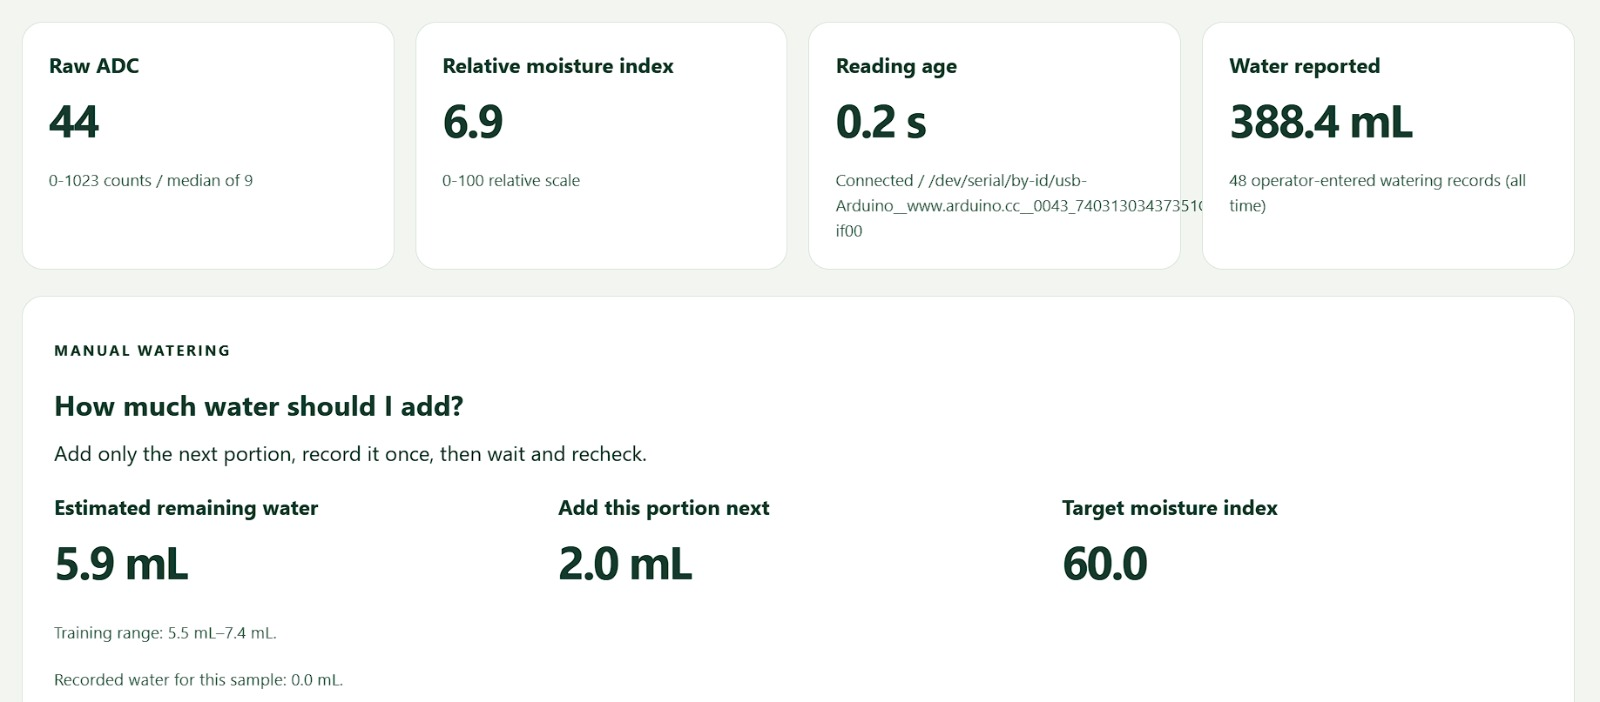
\includegraphics[width=\linewidth,trim=0 0 0 288,clip]{figures/water_prediction.jpeg}
\caption{The water-quantity panel showing the estimated remaining water, next portion and target.}
\label{fig:prediction}
\end{figure}

Four training trials covered the required increase for this example.
Figure~\ref{fig:training-predictions} shows their individual estimates,
which ranged from about 5.5 to 7.4~mL. The median was calculated using
unrounded values and displayed as 5.9~mL. Showing the individual estimates
helped explain how the earlier soil trials contributed to the guidance.
Their variation also supported adding water in small measured portions
and checking the soil response before adding more.

\begin{figure}[htbp]
    \centering
    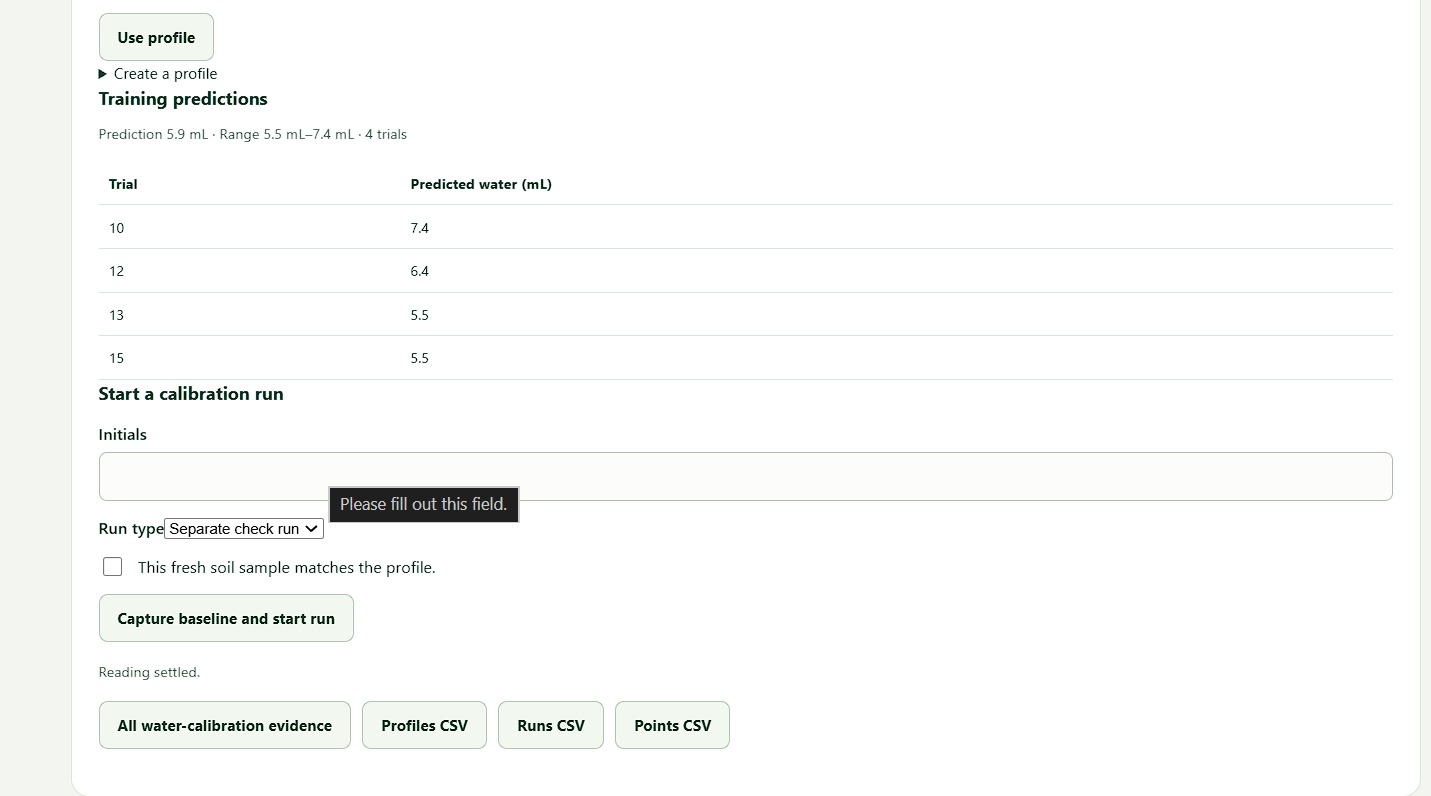
\includegraphics[width=\linewidth,
        trim={90bp 416bp 650bp 80bp},clip]
        {figures/training_predictions.jpeg}
    \caption{Training-curve estimates used for the displayed
    5.9~mL water prediction.}
    \label{fig:training-predictions}
\end{figure}

The total estimate gave the user a useful view of the expected water requirement. The smaller next-portion value turned that estimate into a practical action. Recording each portion and checking the soil again kept the guidance connected to both water use and the measured response.

\subsection{Comparison with a Separate Check Run}

The final method was evaluated by recalculating its estimate from the saved baseline of check run 16. The run started at index 4.7. Applying the final method to that baseline gave approximately 6.1~mL. The saved physical measurements reached index 60.1 after a cumulative 5.5~mL, giving a difference of approximately 0.6~mL between the recalculated estimate and the measured endpoint.

\begin{table}[H]
\centering
\caption{Final-method recalculation using the saved separate check run}
\label{tab:check}
\begin{tabular}{|>{\raggedright\arraybackslash}p{9.4cm}|r|}
\hline
\textbf{Measure} & \textbf{Value} \\ \hline
Starting relative index & 4.7 \\ \hline
Target relative index & 60.0 \\ \hline
Recalculated final-method estimate & 6.1~mL \\ \hline
Measured cumulative water at the final capture & 5.5~mL \\ \hline
Final captured relative index & 60.1 \\ \hline
Difference from measured endpoint & 0.6~mL \\ \hline
\end{tabular}
\end{table}

Figure~\ref{fig:check} shows the watering-response view for this check. It brings together the recorded moisture trace, four water entries and the settled captures. The entries of 2.0, 2.0, 1.0 and 0.5~mL sum to 5.5~mL. The settled index remained below the target at 5.0~mL and reached it after the next 0.5~mL. This supports the use of small final portions and a clear stopping point.

The graph also makes the sequence easier to inspect. The user can see how the index changed around each recorded addition and where a settled capture was taken. Water markers use the entry time, so the measured total and settled captures remain important when interpreting the response.

\begin{figure}[p]
\centering
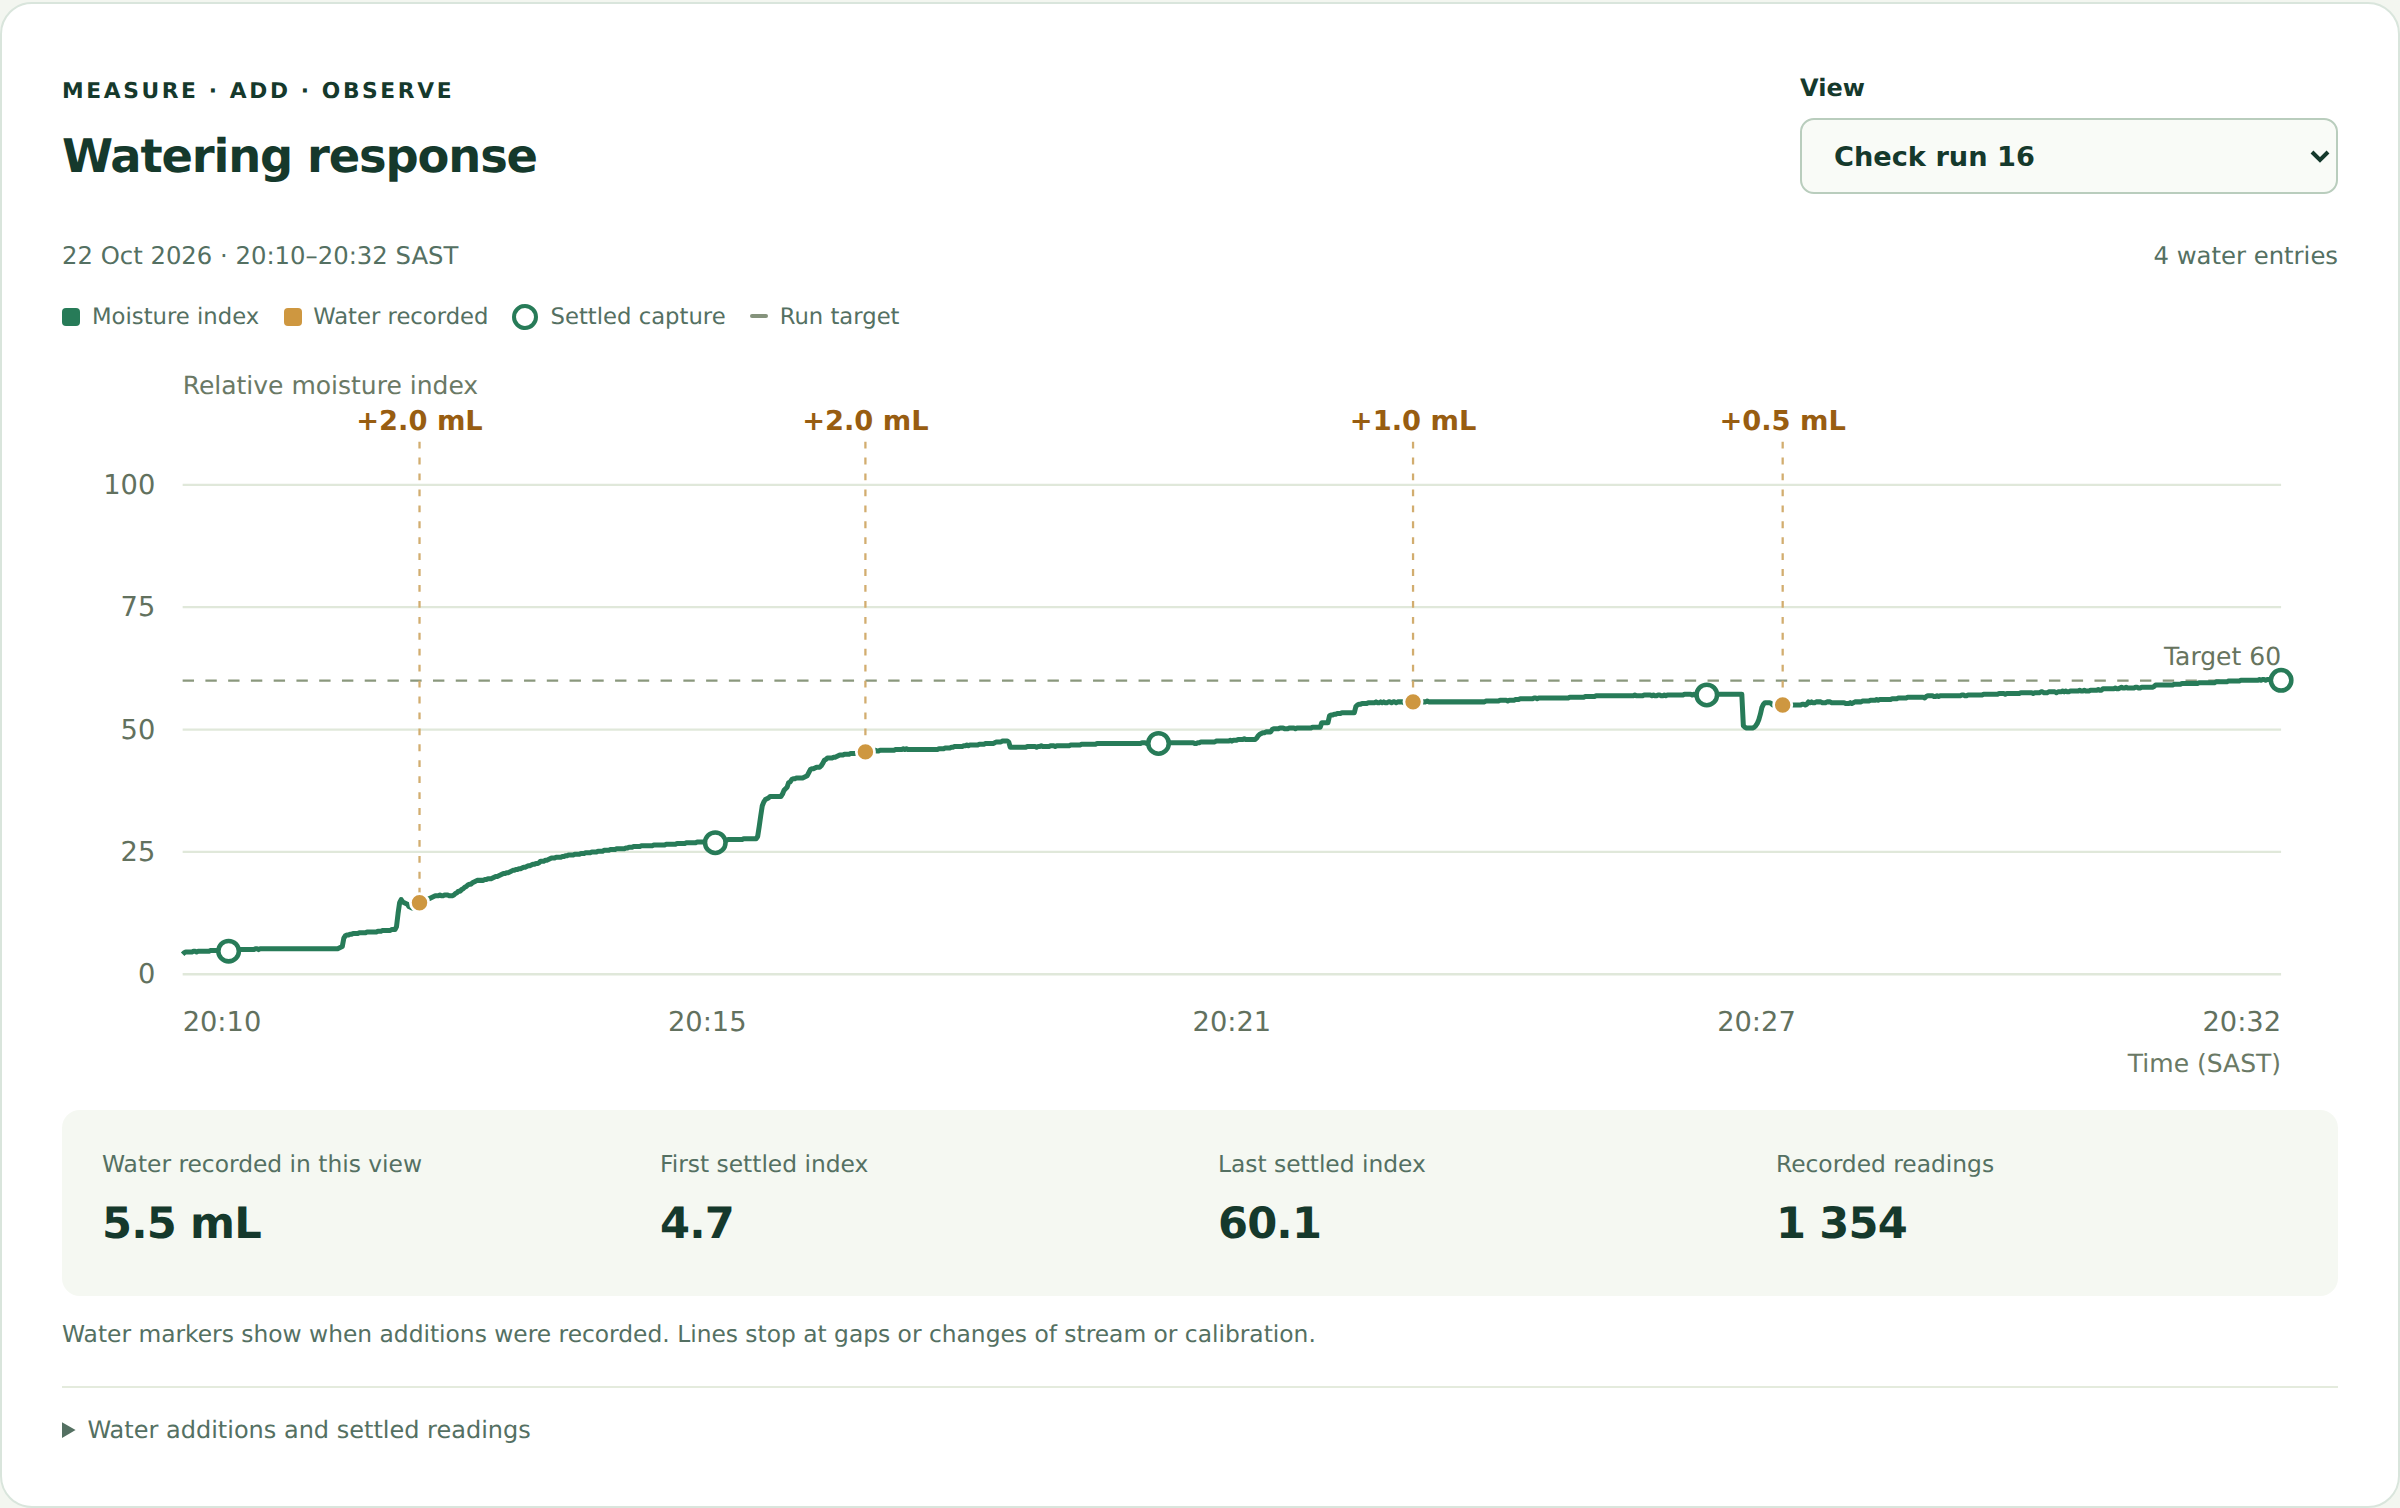
\includegraphics[width=\linewidth]{figures/watering_response.png}
\caption{Watering-response view for check run 16. Four recorded additions total 5.5~mL, and the settled index rises from 4.7 to 60.1.}
\label{fig:check}
\end{figure}

Figure~\ref{fig:prediction-results} presents the same comparison on the prediction-results page. Its saved-recalculation view shows the 6.1~mL estimate beside the 5.5~mL measured total and reports a rounded absolute difference of 0.6~mL. Only one saved recalculation is shown, so its mean and largest differences are equal. These values describe the displayed comparison; further independent checks would establish how consistently the method performs.

\begin{figure}[p]
\centering
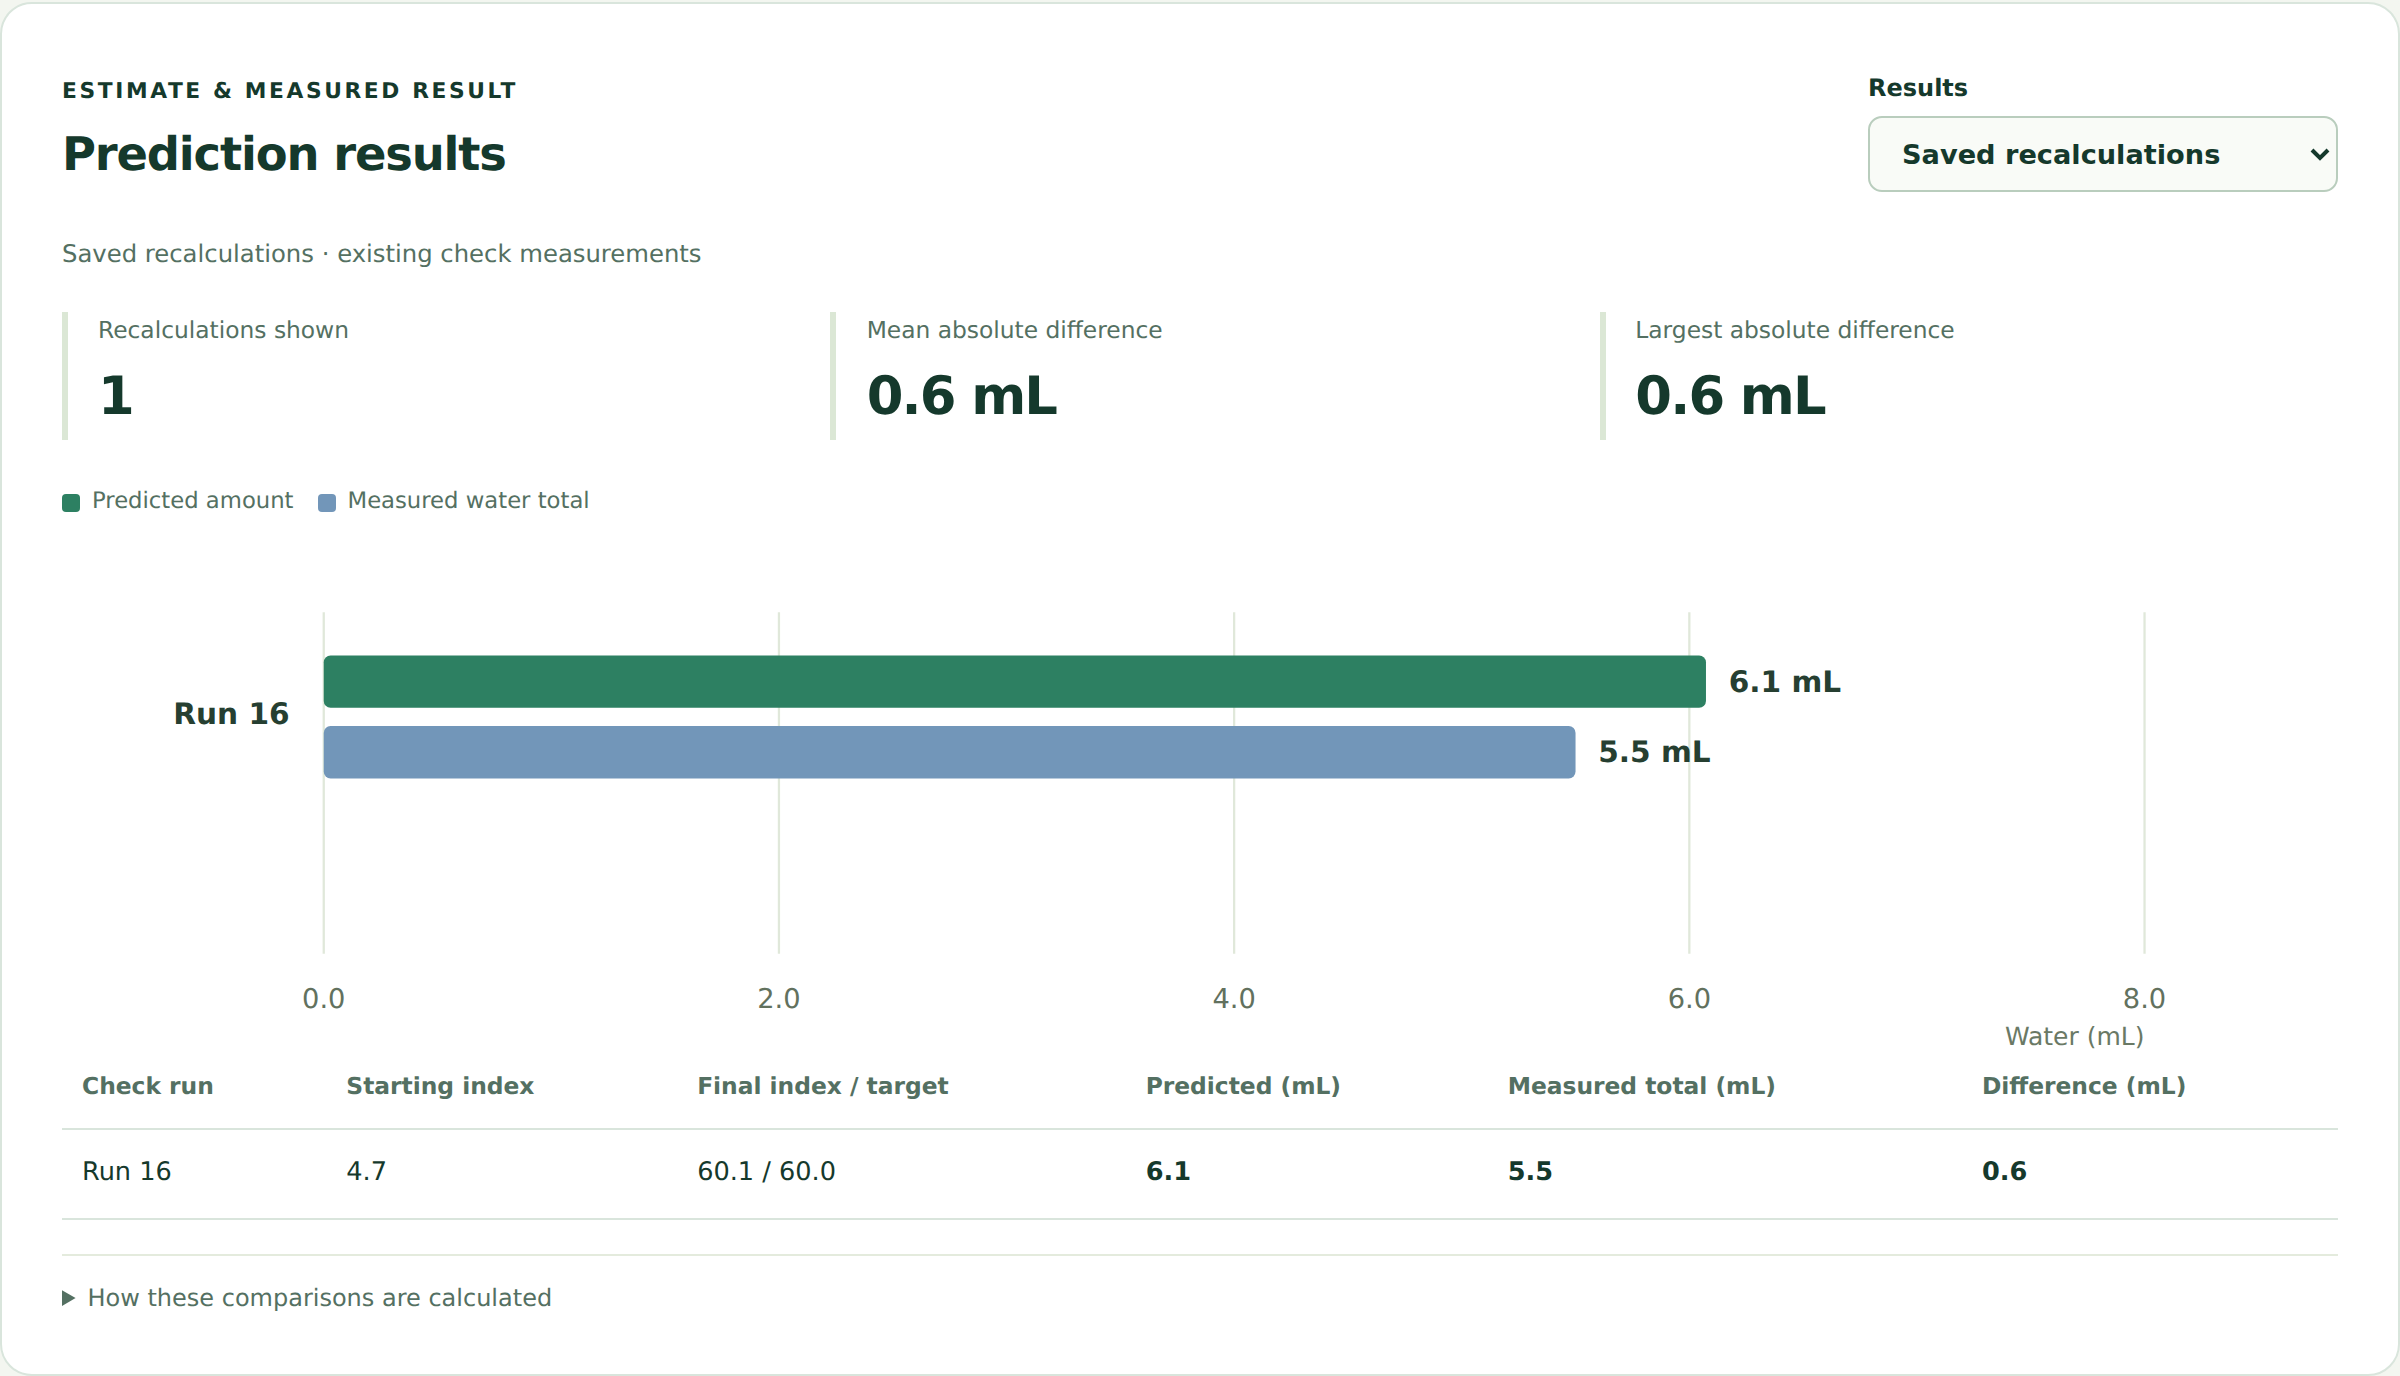
\includegraphics[width=\linewidth]{figures/prediction_results.png}
\caption{Prediction-results view showing the saved recalculation for check run 16, its measured water total and the difference between them.}
\label{fig:prediction-results}
\end{figure}

\Needspace{5\baselineskip}
The comparison uses existing physical measurements to assess the final calculation. The separate-check procedure also allows the system to save a prediction before a fresh watering test begins. The results page makes these records available for inspection alongside the water-response graph.

\FloatBarrier
\subsection{Warnings, Reporting and Recorded Inputs}

The dashboard showed dry-soil warnings under low-index conditions and returned to monitoring once the clearing condition was met. The saved readings demonstrated the three-reading confirmation rule. The visual message and optional browser chime gave the user ways to notice a confirmed dry condition, while the clearing state indicated when the selected moisture level had been reached.

Figure~\ref{fig:monitoring-history} shows how the dashboard displayed
changes in the raw ADC reading and the relative moisture index.
In this example, the index rose gradually towards the clearing level
of 60. The dashed lines mark the warning level of 30 and the clearing
level of 60. These graphs helped the user follow changes in the soil
reading and see how close it was to the selected target.

\begin{figure}[H]
    \centering
    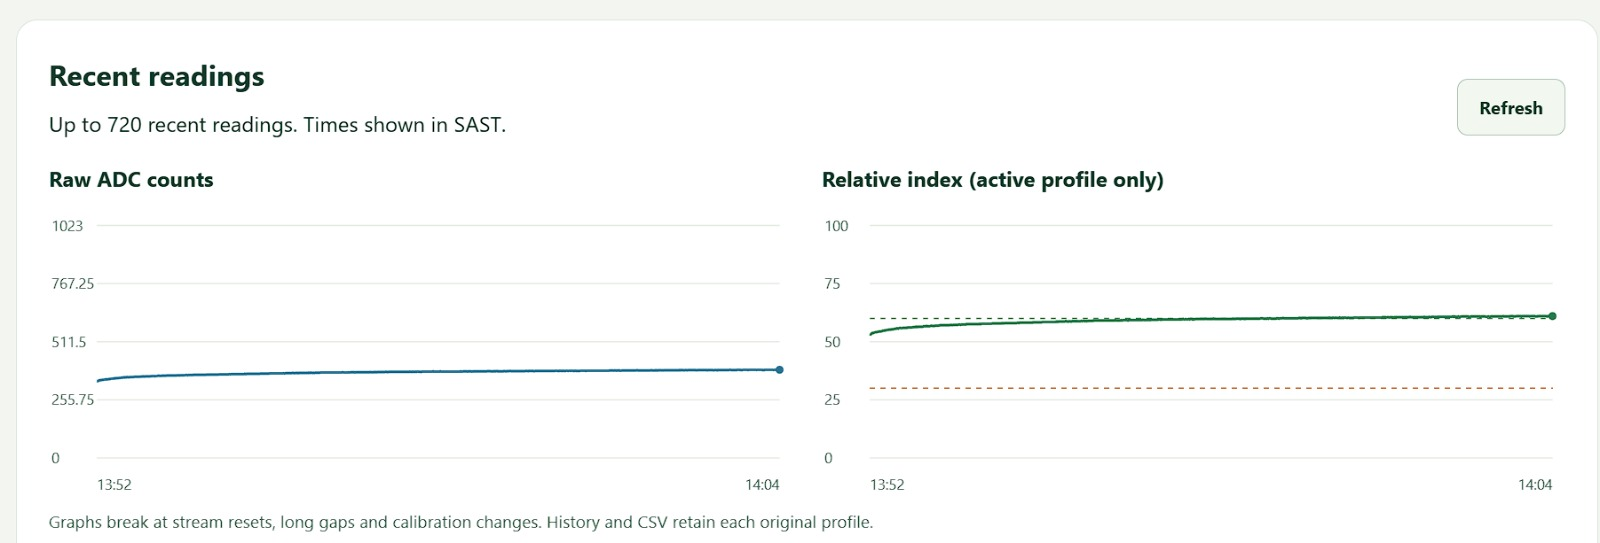
\includegraphics[width=0.9\linewidth,
        trim={25bp 76bp 805bp 157bp},clip]
        {figures/monitoring_history.jpeg}
    \par\medskip
    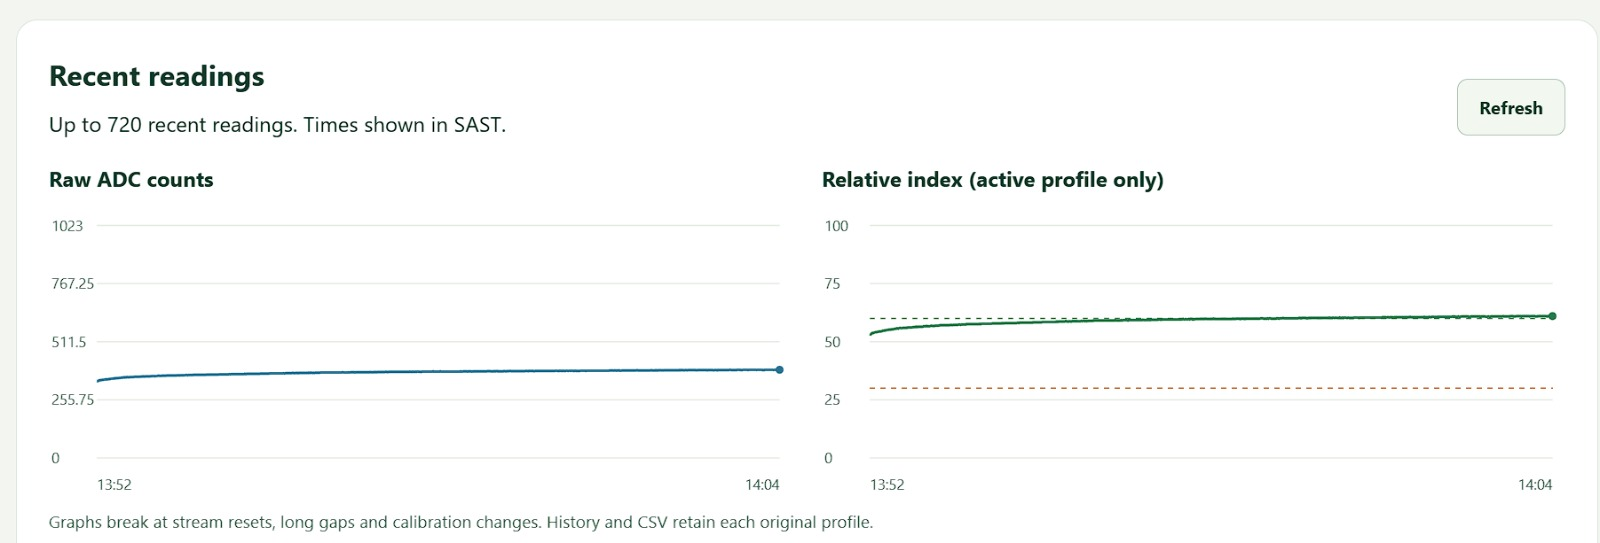
\includegraphics[width=0.9\linewidth,
        trim={815bp 76bp 25bp 157bp},clip]
        {figures/monitoring_history.jpeg}
    \caption{Dashboard graphs showing the raw ADC readings and relative
    moisture index. Earlier readings appear on the left and later readings
    on the right. The dashed lines mark the warning and clearing levels.}
    \label{fig:monitoring-history}
\end{figure}

The five retained training trials used a total of 34.0~mL. The two completed check runs used 12.0~mL, giving 46.0~mL across these quantity-calibration trials. Table~\ref{tab:water} groups the recorded input use. These totals count each physical water addition once, including additions belonging to combined trial sequences.

\begin{table}[htbp]
\centering
\caption{Water recorded for the retained quantity-calibration trials}
\label{tab:water}
\begin{tabular}{|l|c|r|}
\hline
\textbf{Trial group} & \textbf{Number of trials} & \textbf{Water recorded (mL)} \\ \hline
Training & 5 & 34.0 \\ \hline
Separate checks & 2 & 12.0 \\ \hline
Total & 7 & 46.0 \\ \hline
\end{tabular}
\end{table}

The water ledger stored the entered amount with its associated reading. The dashboard displayed cumulative water use, while exports provided the individual entries and trial points. The observation form is used to add notes about visible plant and soil conditions. Together, these features linked the automatic measurements with the user's practical observations and actions.

The recent-readings table provided a direct view of the measurements
behind the graphs. Figure~\ref{fig:recent-readings} shows repeated
readings of 384 ADC and an index of 60.4, together with the recorded
state. This helped the user inspect individual values and compare the
raw sensor output with the calibrated index.

\begin{figure}[htbp]
    \centering
    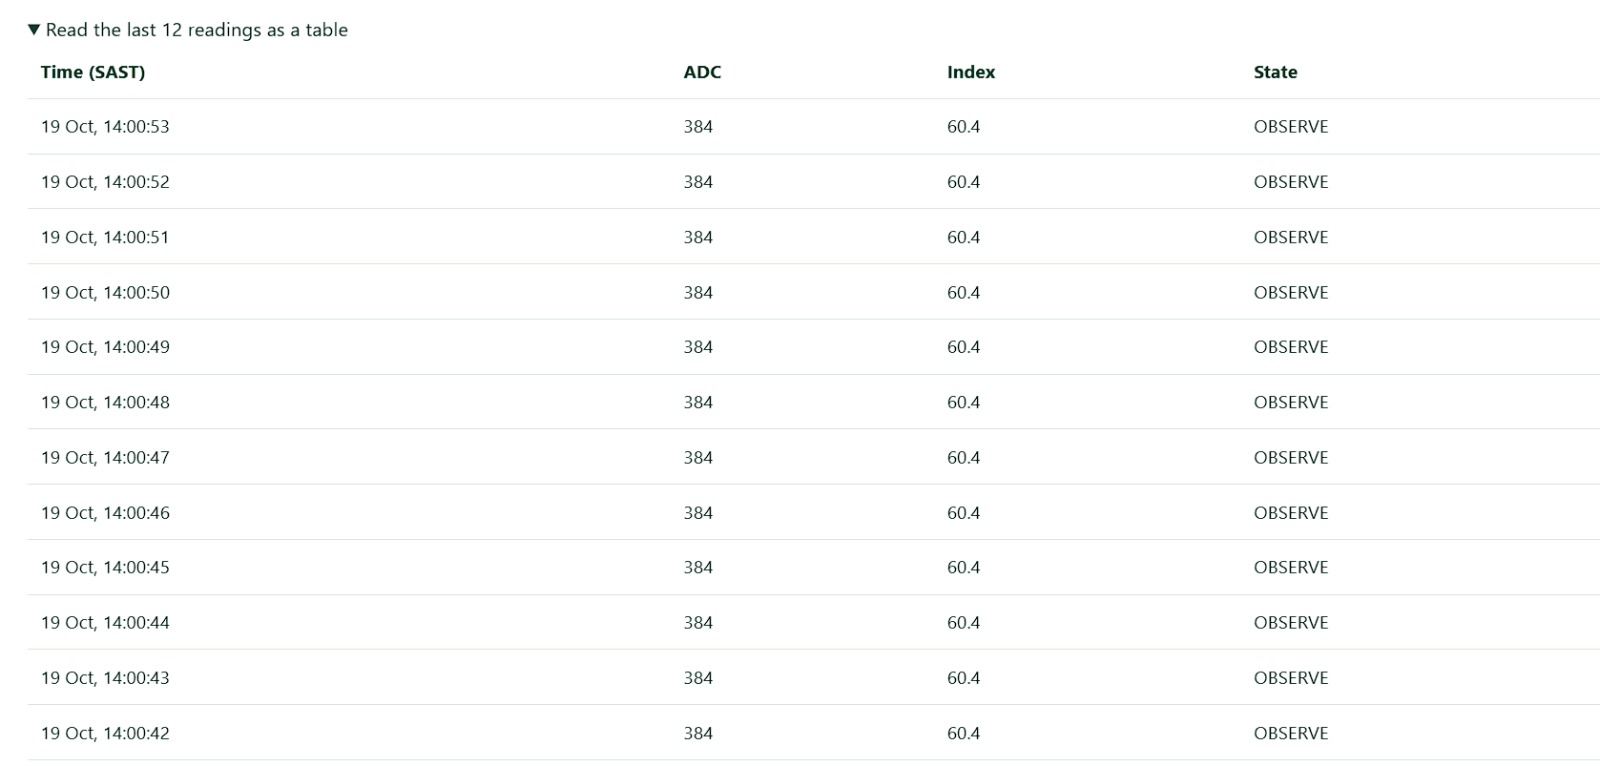
\includegraphics[width=\linewidth,
        trim={640bp 336bp 20bp 47bp},clip]
        {figures/recent_readings.jpeg}
    \caption{An extract from the recent-readings table showing the raw
    ADC value, relative moisture index and recorded state.}
    \label{fig:recent-readings}
\end{figure}

\subsection{Daily and Weekly Water-Use Reporting}

Figure~\ref{fig:water-summaries} shows the daily and weekly summaries from the recorded water ledger. The selected day contains 38.0~mL across 22 water entries, while its calendar week contains 87.4~mL across 45 entries. The weekly bars show how the recorded use is distributed across the days and the saved entry categories.

\begin{figure}[H]
\centering
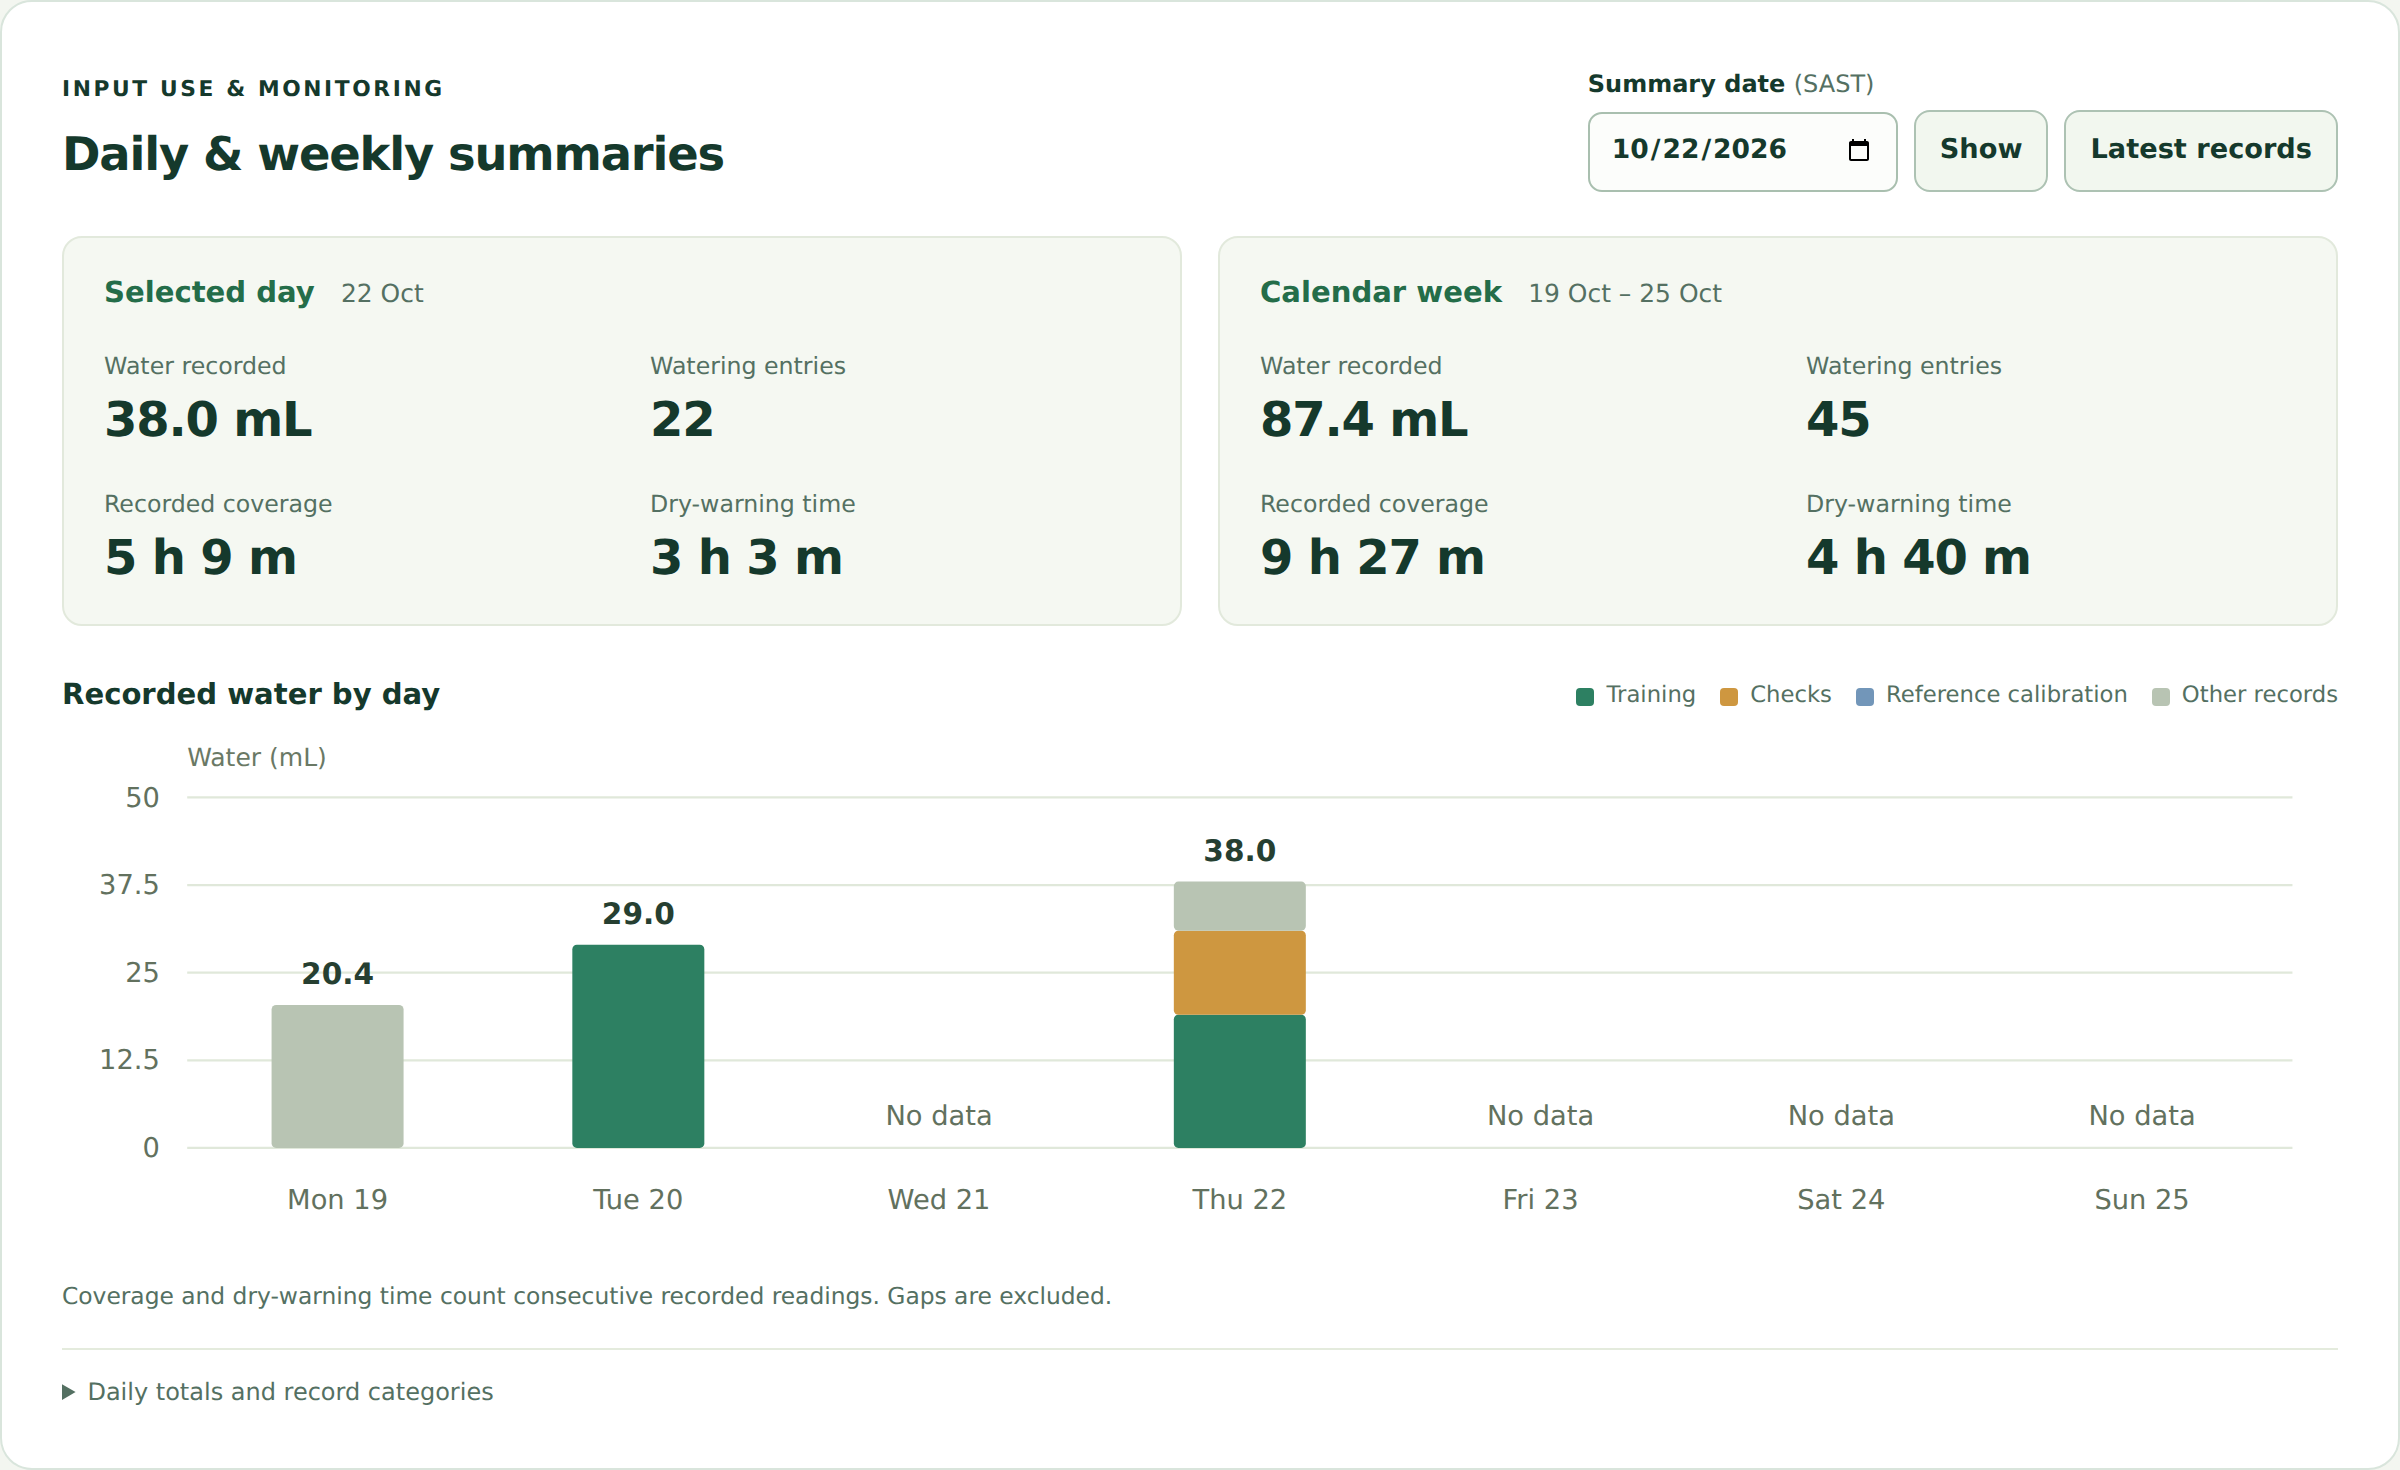
\includegraphics[width=\linewidth]{figures/daily_weekly_summaries.png}
\caption{Daily and weekly summaries showing recorded water use, entry counts, recorded coverage and dry-warning time. The bars group water using the saved entry labels.}
\label{fig:water-summaries}
\end{figure}

These summaries cover all water entries in the selected reporting periods. Table~\ref{tab:water} focuses on the seven retained quantity-calibration trials. The two views answer different practical questions: the trial table reports water used for the retained experimental comparisons, while the summaries report the ledger totals for a chosen period.

Recorded coverage gives context to the warning duration. The totals use consecutive measurements and leave out gaps, so the displayed dry-warning time relates to the periods represented by saved readings. This allows the user to review water use together with the recorded warning history.

The summaries support input reporting by making water use easier to inspect over a day or week. Together with the response and prediction graphs, they connect the amount recorded, the measured soil response and the guidance used during watering.

\subsection{Relationship to the Project Objectives}

The work connected the three objectives through one process: monitor the soil, guide a measured water addition, inspect the response and preserve the record. Table~\ref{tab:objectives} summarises the contribution to each objective.

\begin{table}[htbp]
\centering
\caption{How the implemented functions support the project objectives}
\label{tab:objectives}
\begin{tabular}{|>{\raggedright\arraybackslash}p{4.4cm}|>{\raggedright\arraybackslash}p{10.3cm}|}
\hline
\textbf{Objective} & \textbf{Contribution of the system} \\ \hline
Monitor the garden and guide inputs when needed and in suitable quantities. & Live ADC and relative-index readings report soil condition. Visual and optional audible dry warnings prompt inspection. The trained curves estimate water to reach the target, and the next-portion value guides the measured addition. \\ \hline
Optimise input use, reduce wastage and support crop yield. & Quantity prediction, small portions and a soak pause support careful water use. Response and prediction graphs let the user inspect the measured outcome. Stopping at the target helps maintain growing conditions that favour healthy crops. \\ \hline
Report garden, crop and input conditions. & The dashboard reports moisture, warnings and the clearing state. History graphs link water entries with the soil response and prediction results. Daily and weekly summaries report input use, while observations record crop and soil appearance. \\ \hline
\end{tabular}
\end{table}

The demonstrated functions were live monitoring, warning and clearing behaviour, quantity guidance based on repeated soil trials, water-response and prediction comparisons, and a record of water applied with daily and weekly summaries. These functions provide the measurement and feedback needed for more deliberate water management. The connection to crop growth follows from supporting suitable moisture conditions around the roots \cite{ref14}.

\section{Implementation Experience and Conclusion}

\subsection{Practical Challenges and Exciting Milestones}

The first challenge was connecting the Grove cable to the Uno. Three male-to-male jumpers linked the power, ground and signal wires to the correct sockets. Establishing these connections allowed the Uno to read the probe and send its measurements to the Pi.

Calibration required repeated practical work. The team prepared fresh soil samples, checked the probe placement and repeated water additions while watching the readings settle. An early pair of dry and wet captures was too close to give a useful scale, so the procedure was repeated. The working references became 0 and 636 ADC.

Developing water prediction required a complete record when an early addition produced little visible change. Combining continued sections of the same physical trial preserved the water already applied. Keeping the full response curve, including its starting point, then gave the prediction a clearer basis. Displaying the total estimate alongside the next portion made the result easier to use during watering.

Headless access to the Pi also required troubleshooting hostname and Wi-Fi connections. Working through these problems helped the team understand the path from the physical sensor to the browser. The experience connected wiring, serial communication, data storage, web development and repeated experimental testing.

One of the most exciting milestones was seeing the first live sensor reading appear on the dashboard. Watching the dry warning activate and later clear showed the physical equipment and software working together. It was especially rewarding to see a water estimate generated from the team's own soil trials and displayed as a measurable next portion. These results gave the repeated calibration work a clear purpose and made the prototype feel useful in practice.

\subsection{Equipment Limitations and Future Improvements}

The Grove v1.4 uses exposed metal electrodes. Prolonged electrical contact with wet soil can cause corrosion, changing the probe's response over its working life \cite{ref2}. The electrical path also depends on the soil around the probe. Changes in soil contact and air gaps can affect a reading, so consistent placement remains important \cite{ref4}.

A probe senses a local area. Moisture can vary across a container or garden and at different depths, especially as water spreads through the soil. A set of probes placed at suitable locations and depths would provide broader coverage. A corrosion-resistant capacitive probe is another useful equipment upgrade \cite{refSensorLimits}.

The Uno's ADC represents the signal using discrete digital levels. The syringe also has finite graduations: its 0.5~mL markings determine the portions that can be measured conveniently. These equipment characteristics make sensible rounding and small, measurable additions important.

The Pi and Uno require stable electrical power and secure cable connections. Outdoor use would also benefit from protective housing for the electronics and reliable network coverage for browser access. Future equipment could include a controlled pump and a flow sensor to deliver and verify measured water portions. Further soil trials could compare the response of different probe types and placements.

\subsection{Conclusion}

This project developed a working IoT system that connected soil-moisture monitoring, water-quantity prediction, warning functions and input reporting. The Grove moisture sensor, Arduino Uno and Raspberry Pi 5 supplied live readings to a browser dashboard. The main contribution was linking these readings to practical actions: noticing a dry warning, inspecting the soil, obtaining a water estimate, adding a measured amount and checking the response.

Repeated testing with fresh soil samples was central to this contribution. The moisture calibration gave the ADC readings a consistent relative scale within the tested setup. Further trials linked measured water additions to changes in that index. Five training trials supplied the water-response curves used by the prediction method. This work allowed
the dashboard to provide quantity guidance based on the observed response of the soil and sensor.

The results showed that these training curves could provide a useful initial estimate for the tested conditions. Applying the final method to the saved starting point of a separate check run produced an estimate of 6.1~mL. The measured amount applied to reach the target was 5.5~mL, giving a difference of approximately 0.6~mL. For this check, the estimate was close to the measured total. This supported the use of the training results as a practical starting guide for watering, with further
decisions informed by the soil readings.

The warning rules and watering process gave the prediction a clear purpose. The dry-soil warning prompted the user to inspect the soil and consider whether water was needed. The predicted quantity and suggested next amount helped the user measure each addition. Recording the amount applied allowed the dashboard to track the water remaining from the estimate. The soak pause allowed the water to spread before the next reading was assessed, while the target index provided a stopping point. Together, these features supported careful water use and reduced guesswork during the experiment.

The reporting features formed another important contribution. The watering-response graph linked recorded additions with the moisture trace and settled captures. The prediction-results graph placed estimates beside measured totals, making the difference easy to inspect. Daily and weekly summaries brought water use, recorded coverage and dry-warning time into one view. The observation form provided a place to record visible soil and plant conditions. Together, these features supported immediate watering decisions and later review of the garden's condition and input use.

The project therefore addressed the objectives through three connected functions: monitoring soil conditions, guiding when and how much to water, and reporting the readings and water applied. Its measured watering process provides a practical basis for reducing water wastage and supporting suitable growing conditions.

\clearpage
% IEEE numbered references, ordered by first citation.
\begin{thebibliography}{99}

\bibitem{ref14}
Food and Agriculture Organization of the United Nations, ``Chapter 2: Soil and water.''
[Online]. Available: \url{https://www.fao.org/4/r4082e/r4082e03.htm}

\bibitem{ref4}
University of Minnesota Extension, ``Soil moisture sensors for irrigation scheduling.''
[Online]. Available: \url{https://extension.umn.edu/natural-resources/conservation/agricultural-soil-and-water/irrigation/soil-moisture-sensors-for-irrigation-scheduling}

\bibitem{ref6}
Seeed Studio, ``Grove - Moisture Sensor.''
[Online]. Available: \url{https://wiki.seeedstudio.com/Grove-Moisture_Sensor/}

\bibitem{ref2}
S.~Chowdhury, S.~Sen, and S.~Janardhanan, ``Comparative analysis and calibration of low cost resistive and capacitive soil moisture sensor,'' arXiv:2210.03019, 2022, doi: 10.48550/arXiv.2210.03019.
[Online]. Available: \url{https://arxiv.org/abs/2210.03019}

\bibitem{ref3}
I.~Zaman, N.~Jain, and A.~F{\"o}rster, ``Machine learning based soil VWC and field capacity estimation using low cost sensors,'' arXiv:2102.03354, 2021, doi: 10.48550/arXiv.2102.03354.
[Online]. Available: \url{https://arxiv.org/abs/2102.03354}

\bibitem{ref5}
D.~{\c C}.~Akb{\i}y{\i}k, I.~Mammadova, and E.~Mamishova, ``Soil moisture-based smart irrigation system for efficient water usage in agriculture,'' ResearchGate preprint, 2025, doi: 10.13140/RG.2.2.22576.11525.
[Online]. Available: \url{https://www.researchgate.net/publication/410193444_Soil_Moisture-Based_Smart_Irrigation_System_for_Efficient_Water_Usage_in_Agriculture}

\bibitem{ref9}
Arduino, ``UNO R3.''
[Online]. Available: \url{https://docs.arduino.cc/hardware/uno-rev3/}

\bibitem{ref17}
Raspberry Pi, ``Raspberry Pi computer hardware.''
[Online]. Available: \url{https://www.raspberrypi.com/documentation/computers/raspberry-pi.html}

\bibitem{ref10}
Pallets, ``Waitress, Flask Documentation.''
[Online]. Available: \url{https://flask.palletsprojects.com/en/stable/deploying/waitress/}

\bibitem{ref11}
pySerial contributors, ``pySerial API.''
[Online]. Available: \url{https://pyserial.readthedocs.io/en/latest/pyserial_api.html}

\bibitem{ref12}
Python Software Foundation, ``sqlite3 - DB-API 2.0 interface for SQLite databases.''
[Online]. Available: \url{https://docs.python.org/3/library/sqlite3.html}

\bibitem{refSensorLimits}
Seeed Studio, ``Grove - Capacitive Moisture Sensor (Corrosion Resistant).''
[Online]. Available: \url{https://wiki.seeedstudio.com/Grove-Capacitive_Moisture_Sensor-Corrosion-Resistant/}
\end{thebibliography}

\end{document}
